%%-----------------------------------------------------------------------
% O argumento chapter=TITLE define que todos os títulos de capítulos
% saiam em caixa alta (maiúsculas). Se não quiser caixa alta, basta
% remover este argumento.
\documentclass[12pt,oneside,a4paper,chapter=TITLE,
			   english,brazil]{abntex2}


%%-----------------------------------------------------------------------
% Carregando a padronização para a capa, contra-capa e folha de
% assinaturas adotada pela UEPB
\usepackage{TCC_UEPB}
\usepackage{graphicx}
\usepackage{sectsty}
%\pagenumbering{arabic}
%%-----------------------------------------------------------------------
% Pacotes básicos 
\usepackage{mathptmx}		% Usa a fonte Times New Roman
\usepackage[T1]{fontenc}	% Selecao de codigos de fonte.
\usepackage[utf8]{inputenc}	% Cod. do doc. (conversão autom. dos acentos)
\usepackage{lastpage}		% Usado pela Ficha catalográfica
\usepackage{indentfirst}	% Indenta o primeiro parágrafo de cada seção.
\usepackage{float}
\usepackage{forest}
\usepackage{color}			% Controle das cores
\usepackage{graphicx}		% Inclusão de gráficos
\usepackage{microtype} 		% para melhorias de justificação
\usepackage{pdfpages}		% para a inclusão de documentos em PDF.
\usepackage{multirow}       % VARIAS LINHAS NA TABELA
\usepackage{colortbl}       % CORES NA TABELA
\usepackage{hyperref}
\usepackage{titlesec}
%%------------------------------------------------------------------------
% Pacotes adicionais, para definir ambientes para definição, teorema 
% e axioma. Outros ambientes podem ser definidos da mesma forma...
\usepackage{amssymb}     % qed
\usepackage{amsthm}      % Teoremas
\usepackage{amsmath}     % Para o ambiente align (alinhar equações)
\usepackage{thmtools}    % Front end para amsthm (\declaretheorem)
%\usepackage{parskip}
%\usepackage{titlesec}
\usepackage{hyperref}

%%-----------------------------------------------------------------------
% Definição de ambientes para definição, teorema, etc...
\declaretheorem[style=definition,name=Definição,qed=\textemdash]{definicao}
\declaretheorem[style=plain,name=Teorema,qed=\textnormal{\textemdash}]{teorema}
\declaretheorem[style=plain,name=Axioma,qed=\textnormal{\textemdash}]{axioma}
\declaretheorem[style=plain,name=Lema,qed=\textnormal{\textemdash}]{lema}
% Configuração para seções e subseções
%\titleformat{\section}{\normalfont\Large\bfseries}{\thesection}{1em}{}
\titleformat{\subsection}{\normalfont\large\bfseries}{\thesubsection}{1em}{}

% configurando seções 



%%------------------------------------------------------------------------
% Pacotes de citações
\usepackage[brazilian,hyperpageref]{backref} % Página citada na bibliog.
\usepackage[alf]{abntex2cite}				 % Citações padrão ABNT

%\titlespacing{\chapter}{0pt}{*0}{*0}
%\titlespacing{\section}{0pt}{*0}{*0}
%%-----------------------------------------------------------------------
%% CONFIGURAÇÕES DE PACOTES
%%-----------------------------------------------------------------------

\usepackage{fancyhdr}
\usepackage[bottom=2cm,top=2cm]{geometry} % Ajusta as margens

\pagestyle{plain} % Configura o estilo de página para plain

\fancypagestyle{plain}{%
  \fancyhf{} % Limpa todos os cabeçalhos e rodapés
  \renewcommand{\headrulewidth}{0pt} % Remove a linha do cabeçalho
  \fancyhead[R]{\raisebox{2cm}{\thepage}} % Ajusta a posição vertical (aumentado para -2cm)
}
%%-----------------------------------------------------------------------
% Configurações do pacote backref Usado sem a opção hyperpageref
% de backref
\renewcommand{\backrefpagesname}{Citado na(s) página(s):~}
% Texto padrão antes do número das páginas
\renewcommand{\backref}{}   % Define os textos da citação
\renewcommand*{\backrefalt}[4]{
	\ifcase #1 %
	Nenhuma citação no texto.%
	\or
	Citado na página #2.%
	\else
	Citado #1 vezes nas páginas #2.%
	\fi}%


%%----------------------------------------------------------------------
% Configurações de aparência do PDF final
\makeatletter
\hypersetup{     % informações do PDF
	pdftitle={\@title}, 
	pdfauthor={\@author},
	pdfsubject={\imprimirpreambulo},
	colorlinks=true,   % false: box links; true: color links
	linkcolor=black,   % color of internal links
	citecolor=black,   % color of links to bibliography
	filecolor=black,   % color of file links
	urlcolor=black,    % color of url links
	bookmarksdepth=4
}
\makeatother


%%------------------------------------------------------------------
% Cria uma nova série (de símbolos) para footnotes
\newcounter{savefootnote}
\newcounter{symfootnote}
\newcommand{\symfootnote}[1]{%
	\setcounter{savefootnote}{\value{footnote}}%
	\setcounter{footnote}{\value{symfootnote}}%
	\ifnum\value{footnote}>8\setcounter{footnote}{0}\fi%
	\let\oldthefootnote=\thefootnote%
	\renewcommand{\thefootnote}{\fnsymbol{footnote}}%
	\footnote{#1}%
	\let\thefootnote=\oldthefootnote%
	\setcounter{symfootnote}{\value{footnote}}%
	\setcounter{footnote}{\value{savefootnote}}%
}


% remove informações do  top das paginas 


%\pagestyle{empty} 

%%-----------------------------------------------------------------------
% Informações de dados para CAPA, FOLHA DE ROSTO e FOLHA DE APROVAÇÃO
\titulo{ PREDIÇÃO DA SÍNDROME RESPIRATÓRIA AGUDA GRAVE POR MEIO DE MULTICLASSIFICAÇÃO COM ALGORITMOS DE MACHINE LEARNING}   % Subtítulo apenas se houver
\tituloestrangeiro{PREDICTION OF SEVERE ACUTE RESPIRATORY SYNDROME THROUGH MULTICLASSIFICATION USING MACHINE LEARNING ALGORITHMS} % Title (English - opcional)
\autor{JOSEFERSON DA SILVA BARRETO}   % Digite seu nome aqui
\local{Campina Grande - PB}
\data{2023}                              % Na data coloque apenas o ano
\orientador[Prof. Dr.]{%Ricardo Alves de Olinda & \\
            Tiago Almeida de Oliveira} % Nome do orientador aqui
%\coorientador[]{} % Coorientador (se tiver)

%%-----------------------------------------------------------------------
% Informações sobre campus, centro, depto e curso
% \campus e \curso são obrigatórios e precisam ser preenchidos!!
% Todos os demais são opcionais (para o LaTeX), pois note que o 
% \preambulo é exigido pela Biblioteca na entrega do trabalho.
\campus{Campus I - CAMPINA GRANDE}
\centro{Centro de Ciências e Tecnologia}
\depto{Departamento de Estatística}
\curso{CURSO DE GRADUAÇÃO EM BACHARELADO EM ESTATÍSTICA}
\tipotrabalho{Trabalho de Conclusão de Curso}
\preambulo{
  Trabalho de Conclusão de Curso apresentado ao curso de Bacharelado em Estatística do Departamento de Estatística do Centro de Ciências e Tecnologia da Universidade Estadual da Paraíba, como requisito parcial à obtenção do título de bacharel em Estatística.
}


%%-----------------------------------------------------------------------
% compila o indice
\makeindex

\usepackage{pdfpages}

%\pagestyle{plain}

%%-----------------------------------------------------------------------
%%      INÍCIO DO DOCUMENTO
%%-----------------------------------------------------------------------

\setlength{\absparsep}{18pt}
\begin{document}


% Retira espaço extra obsoleto entre as frases.
\frenchspacing 


%%-----------------------------------------------------------------------
% ELEMENTOS PRÉ-TEXTUAIS
\pretextual


%%------------------------------------------------------------------------
% Capa
\imprimircapa


%%-----------------------------------------------------------------------
% Folha de rosto
\imprimirfolhaderosto
%%-----------------------------------------------------------------------
% Inserir a ficha bibliografica (depois de feita pela Biblioteca e salva 
% em PDF). Descomentar as 4 linhas abaixo.
%\begin{fichacatalografica}
  %  \includepdf{Ficha-Catalografica-172090776.pdf}
%\end{fichacatalografica}
%setcounter{page}{2}

\includepdf{Ficha-Catalografica-172090776.pdf}

\setcounter{page}{2} % Define o contador de páginas

%%------------------------------------------------------------------------
% Inserir folha de aprovação
\setlength{\ABNTEXsignwidth}{8cm}    % Comp. da linha de assinaturas 
\membroum[Prof. Dr.]{Tiago Almeida de Oliveira(Orientador) %& Prof. Dr.Ricardo Alves de Olinda (Orientador) \\
	Universidade Estadual da Paraíba (UEPB)}
\membrodois[Prof. Dr.]{Ricardo Alves de Olinda \\ 
	Universidade Estadual da Paraíba (UEPB)}
    
%\membrotres%[%Prof. Dr.]
%{%nome \\ 
%	Universidade Federal... (UFMT)
 %Ednário Mendonça}
 \membrotres[Prof. Me.]{Cleanderson Romualdo Fidelis \\
   Universidade Estadual da Paraíba (UEPB)}
\datadefesa{13/07/2023}
\folhadeaprovacaoUEPB

%%-----------------------------------------------------------------------       
%%                         IMPORTANTE!!
% Após a defesa digitalize a folha de aprovação em um arquivo PDF, co-
% mente as 9 linhas acima e acrescente o PDF digitalizado descomentando
% a linha a seguir:
%\includepdf{folha_aprovacao.pdf}


%%-----------------------------------------------------------------------
%                Dedicatória (OPCIONAL)
% Comente as linhas abaixo se não quiser usar.
\begin{dedicatoria}
	\vspace*{\fill}
	\hspace{.45\textwidth}
	\begin{minipage}{.5\textwidth}
   		Dedico este trabalho a Deus, minha família, amigos e colegas que estiveram sempre juntos comigo durante toda minha jornada acadêmica.
	\end{minipage}
\end{dedicatoria}


%%-----------------------------------------------------------------------
%              Agradecimentos (OPCIONAL)
% Comente as linhas abaixo se não quiser usar.
\begin{agradecimentos}
Gostaria de expressar meu sincero agradecimento a todas as pessoas que contribuíram para a conclusão bem-sucedida deste trabalho de conclusão de curso. Neste momento especial, desejo expressar minha gratidão a Deus, minha família, amigos, colegas e meu orientador, além dos professores que estiveram ao meu lado durante essa jornada. Em primeiro lugar, agradeço a Deus por me conceder a força, a sabedoria e a perseverança necessárias para superar os desafios ao longo deste processo. Sua orientação e apoio constantes foram fundamentais para alcançar esse marco importante em minha vida acadêmica.

À minha família, meu porto seguro, expresso minha profunda gratidão. O amor, o incentivo e o apoio incondicionais que recebi de meus pais, irmãos e outros familiares foram cruciais para me manter motivado e focado em meus objetivos. Vocês sempre acreditaram em mim e me encorajaram a nunca desistir, mesmo nos momentos mais difíceis. Sou imensamente grato por ter vocês ao meu lado. Aos meus amigos e colegas, sou grato por compartilharmos essa jornada acadêmica juntos. Agradeço por todas as trocas de conhecimento, apoio mútuo, estudo em grupo e momentos de descontração que compartilhamos ao longo dos anos. Vocês tornaram essa jornada mais leve e memorável. Sou grato pela amizade e pelo suporte inestimável que me proporcionaram.

Ao meu orientador, expresso minha sincera gratidão pela sua orientação, conhecimento e dedicação ao longo do processo de desenvolvimento deste trabalho. Suas orientações valiosas, sugestões e críticas construtivas foram fundamentais para moldar este projeto. Agradeço por ter compartilhado seu tempo, conhecimento e experiência comigo. Sou imensamente grato pela sua paciência e pela confiança que depositou em meu trabalho.

Também quero estender meu agradecimento a todos os professores que contribuíram para a minha formação acadêmica. Suas aulas, orientações e ensinamentos foram fundamentais para meu crescimento intelectual e profissional. Sou grato por ter tido a oportunidade de aprender com profissionais tão dedicados e experientes.

Por fim, gostaria de expressar minha gratidão a todos aqueles que, de alguma forma, contribuíram para o meu sucesso nesta jornada. Seja através de palavras de encorajamento, apoio emocional ou assistência prática, cada gesto foi importante e significativo.Este trabalho não teria sido possível sem a presença de todas essas pessoas especiais em minha vida. Agradeço do fundo do coração por todo o apoio, incentivo e confiança que recebi ao longo dessa jornada. Sinto-me verdadeiramente abençoado por ter cada um de vocês ao meu lado. O meu mais sincero obrigado a Deus, à minha família, amigos, colegas, orientador e professores. Vocês foram essenciais para a minha conquista acadêmica e sou eternamente grato por tudo o que fizeram por mim.
\end{agradecimentos}


%%-----------------------------------------------------------------------
%                  Epígrafe  (OPCIONAL)
% Comente as linhas abaixo se não quiser usar.
\begin{epigrafe}
    \vspace*{\fill}
	\begin{flushright}
		``O senhor é meu pastor e nada me faltará!'' \\
	                             (Salmo 23)
	\end{flushright}
\end{epigrafe}


%%------------------------------------------------------------------------
%                           RESUMOS
% O resumo em português é obrigatório, seguido da sua versão em outro 
% idioma, que pode ser inglês (mais comum), francês ou espanhol.

% resumo em português (OBRIGATÓRIO)
\setlength{\absparsep}{18pt} % ajusta espaçamento de parág. do resumo
\begin{resumo}

%A Síndrome Respiratória Aguda Grave (SRAG) é uma condição médica grave que afeta os pulmões e o sistema respiratório. Ela é caracterizada por sintomas como febre alta, tosse, falta de ar e dificuldade respiratória. A SRAG pode ser causada por uma variedade de vírus, incluindo o coronavírus SARS-CoV-2, que causa a COVID-19. Além disso, ela é uma condição que pode levar a complicações graves, como pneumonia e insuficiência respiratória, e pode exigir hospitalização e cuidados intensivos. Em casos mais graves, a síndrome pode resultar em insuficiência de múltiplos órgãos e levar à morte. A SRAG é especialmente preocupante devido à sua capacidade de se espalhar facilmente de pessoa para pessoa. Em surtos epidêmicos, como o caso da pandemia de COVID-19, a SRAG pode se disseminar rapidamente, colocando um grande número de pessoas em risco de contrair a doença.  O diagnóstico  é feito com base na avaliação dos sintomas clínicos, exames de imagem dos pulmões e testes laboratoriais para identificar o agente causador. A utilização de modelos de machine learning para analisar a Síndrome Respiratória Aguda Grave (SRAG) pode trazer importantes benefícios no contexto da saúde pública e da medicina. Aqui estão algumas razões pelas quais esses modelos são importantes: detecção precoce, classificação de gravidade, prognóstico e tratamento entre outras. 


A Síndrome Respiratória Aguda Grave (SRAG) é uma condição médica grave que afeta o sistema respiratório, causando sintomas como febre alta, tosse, falta de ar e dificuldade respiratória. Sua etiologia pode ser diversa, incluindo o coronavírus SARS-CoV-2, responsável pela COVID-19. A SRAG pode levar a complicações graves, como pneumonia e insuficiência respiratória, demandando cuidados hospitalares intensivos e, em casos mais graves, pode resultar em insuficiência de múltiplos órgãos e morte. Este trabalho teve como objetivo demonstrar algumas das principais técnicas de \textit{Machine Learning} para a classificação multiclasse de SRAG, visando aprimorar a capacidade de previsão da síndrome. Para isso, foram utilizados diferentes modelos de classificação, voltados especificamente para classificação multiclasse. Os resultados obtidos revelaram que o modelo XGBoost se destacou, alcançando uma performance geral de 83\%. Esse modelo apresentou excelentes resultados na classificação de SRAG por influenza, SRAG por Covid e outras SRAGs relacionadas a vírus respiratórios. No entanto, identificou-se um desempenho razoável nas classes 3 e 4, que representam SRAG por outros agentes etiológicos e um tipo não especificado de SRAG, respectivamente. Esses resultados reforçam a importância do uso de técnicas de \textit{Machine Learning} na análise da SRAG, contribuindo para melhorar a capacidade de previsão e diagnóstico da síndrome. Futuras pesquisas podem se concentrar em aprimorar o desempenho do modelo nas classes mais desafiadoras, buscando aperfeiçoar a aplicação prática dessas técnicas na saúde pública e na medicina.
 
	\textbf{Palavras-chave}: previsão de SRAG; saúde pública;  modelos de aprendizado de máquina; classificação multiclasse.
	% Número máximo de 4 palavras-chave.
\end{resumo}

% resumo em inglês(OBRIGATÓRIO)
\begin{resumo}[Abstract]
	\begin{otherlanguage*}{english}
%Severe Acute Respiratory Syndrome (SARS) is a serious medical condition that affects the lungs and the respiratory system. It is characterized by symptoms such as high fever, cough, shortness of breath, and difficulty breathing. SARS can be caused by a variety of viruses, including the SARS-CoV-2 coronavirus, which causes COVID-19. Additionally, it is a condition that can lead to severe complications such as pneumonia and respiratory failure, requiring hospitalization and intensive care. In severe cases, the syndrome can result in multiple organ failure and death. SARS is particularly concerning due to its ability to easily spread from person to person. During epidemic outbreaks, such as the COVID-19 pandemic, SARS can rapidly spread, putting a large number of people at risk of contracting the disease. Diagnosis is based on the assessment of clinical symptoms, lung imaging tests, and laboratory tests to identify the causative agent. The use of machine learning models to analyze Severe Acute Respiratory Syndrome (SARS) can bring significant benefits in the context of public health and medicine. Here are some reasons why these models are important: early detection, severity classification, prognosis, and treatment, among others.


Acute Severe Respiratory Syndrome (ASRS) is a severe medical condition that affects the respiratory system, causing symptoms such as high fever, cough, shortness of breath, and respiratory distress. Its etiology can be diverse, including the SARS-CoV-2 coronavirus, responsible for COVID-19. ASRS can lead to serious complications such as pneumonia and respiratory failure, requiring intensive hospital care and, in severe cases, can result in multiple organ failure and death. This study aimed to demonstrate some of the main machine learning techniques for multiclass classification of ASRS, aiming to improve the syndrome's predictive capability. Different classification models specifically tailored for multiclass classification were used to achieve this goal. The results obtained revealed that the XGBoost model stood out, achieving an overall performance of 83\%. This model showed excellent results in classifying ASRS caused by influenza, ASRS caused by Covid, and other ASRS related to respiratory viruses. However, reasonable performance was identified in classes 3 and 4, representing ASRS caused by other etiological agents and an unspecified type of ASRS, respectively. These results reinforce the importance of using machine learning techniques in ASRS analysis, contributing to improving the predictive capability and diagnosis of the syndrome. Future research can focus on enhancing the model's performance in the more challenging classes, seeking to refine the practical application of these techniques in public health and medicine.
		
		%\textbf{Keywords}: ASRS prediction. Machine Learning. Multiclassification.
        
        \textbf{Keywords}: ASRS prediction; public health; machine learning models; multiclass classification.
	\end{otherlanguage*}
\end{resumo}
\vspace{\onelineskip}


%%-----------------------------------------------------------------------
%              inserir lista de ilustrações (OPCIONAL)
% Comente as linhas abaixo se não quiser usar.
\pdfbookmark[0]{\listfigurename}{lof}
\listoffigures*
\cleardoublepage


%%-----------------------------------------------------------------------
%              inserir lista de tabelas (OPCIONAL)
% Comente as linhas abaixo se não quiser usar.
\pdfbookmark[0]{\listtablename}{lot}
\listoftables*
\cleardoublepage

%%-----------------------------------------------------------------------
%           Inserir o Sumario


\pdfbookmark[0]{\contentsname}{toc}
\tableofcontents*
\cleardoublepage


%%-----------------------------------------------------------------------
%        ELEMENTOS TEXTUAIS
\textual

\setcounter{page}{12}
%%-----------------------------------------------------------------------
%                             Introdução
\chapter{Introdução}
\label{introducao}

 A Síndrome Respiratória Aguda Grave (SRAG),   é  condição clínica caracterizada por sintomas respiratórios graves que exigem hospitalização e pode ser causada por uma variedade de agentes infecciosos, como vírus, bactérias ou fungos. Ela geralmente se manifesta como uma infecção do trato respiratório inferior, afetando os pulmões e causando sintomas como febre alta, tosse persistente, falta de ar, dor no peito e dificuldade respiratória. Em casos mais graves, a SRAG pode levar à insuficiência respiratória e exigir suporte ventilatório. De acordo com \citeonline{minsaude} são sintomas do SARGS: indivíduo com  síndrome gripal (SG) que apresente: dispneia/desconforto respiratório ou pressão ou dor persistente no tórax ou saturação de  oxigênio (O2) menor que 95\% em ar ambiente ou coloração azulada (cianose) dos lábios ou rosto.  Vale salientar, no entanto, que nem todos os casos da síndrome são explicados pela infecção por Sars-CoV-2, pois, como mencionado, outras infecções respiratórias podem desencadear o problema \cite{brasilescola}.



Segundo \citeonline{juca}, nos últimos anos, o surgimento da Covid-19 e o aumento no número de casos de gripe geraram uma atmosfera de medo e incertezas. Essa situação é agravada pela semelhança entre os sintomas de diferentes síndromes respiratórias graves, tornando a classificação e o diagnóstico um desafio para os profissionais de saúde. Muitas dessas síndromes compartilham sintomas comuns, como febre, tosse, falta de ar e dor no peito, resultando em uma sobreposição de características clínicas que pode dificultar a identificação precisa da doença em questão.

A importância do \textit{Machine Learning} vem crescendo nos últimos anos, impulsionada pelo aumento na disponibilidade de dados, pela evolução dos algoritmos de aprendizagem e pelo avanço da capacidade de processamento dos computadores. Com isso, tornou-se possível realizar análises cada vez mais sofisticadas e precisas em áreas como finanças, marketing, saúde, entre outras. O uso de técnicas de \textit{Machine Learning} proporciona uma abordagem inovadora para lidar com a complexidade dos dados relacionados à SRAG, permitindo que padrões  sejam identificados. Essas técnicas explorarão os dados existentes, como informações clínicas, resultados de exames laboratoriais e históricos médicos, a fim de construir um modelo preditivo capaz de auxiliar na identificação correta do tipo de SRAG.  



Nesta monografia, o objetivo é desenvolver um modelo de classificação eficaz utilizando técnicas de aprendizado de máquina \textit{Machine Learning} para identificar e classificar corretamente os diferentes tipos de Síndrome Respiratória Aguda Grave (SRAG). Para alcançar esse objetivo, será empregado o uso de algoritmos de \textit{Machine Learning} que analisarão dados clínicos e epidemiológicos relevantes. O intuito é criar um modelo preditivo capaz de distinguir entre os tipos específicos de SRAG de forma mais precisa e eficiente.


%Compreender o processo de \textit{Machine Learning}  é essencial para entender as tecnologias que impulsionam a Inteligência Artificial. O \textit{Machine Learning} é um ramo da computação que busca criar modelos estatísticos capazes de aprender a realizar tarefas sem serem explicitamente programados para isso. Ao usar algoritmos para analisar dados, o \textit{Machine Learning} pode automatizar a tomada de decisões e fornecer insights úteis a partir de grandes conjuntos de dados.

%A importância do \textit{Machine Learning} vem crescendo nos últimos anos, impulsionada pelo aumento na disponibilidade de dados, pela evolução dos algoritmos de aprendizagem e pelo avanço da capacidade de processamento dos computadores. Com isso, tornou-se possível realizar análises cada vez mais sofisticadas e precisas em áreas como finanças, marketing, saúde, entre outras.


%Nesta monografia, utilizaremos técnicas de aprendizado de máquina (machine learning) com o objetivo de melhorar a predição do tipo de Síndrome Respiratória Aguda Grave (SRAG).

%Nesta monografia, o objetivo é desenvolver um modelo de classificação utilizando técnicas de aprendizado de máquina (machine learning) para a correta identificação e classificação dos diferentes tipos de Síndrome Respiratória Aguda Grave (SRAG).
%A proposta é empregar algoritmos de machine learning para analisar dados clínicos e epidemiológicos, a fim de desenvolver um modelo preditivo mais eficaz na identificação do tipo específico de SRAG.





%Nas próximas páginas, apresentaremos uma introdução ao Machine Learning, abordando seus principais conceitos e técnicas, além de destacar alguns de seus principais usos na atualidade.

%Capítulo 1: O que é Machine Learning?

%Neste capítulo, apresentaremos uma breve introdução sobre o que é Machine Learning e sua importância no cenário do mundo atual.

%Capítulo 2: Material e Métodos

%Neste capítulo,apresentaremos os materiais e métodos utilizados para aplicar as técnicas de machine learning na classificação de síndromes gripais agudas. Nesta seção, descreveremos detalhadamente os passos e recursos necessários para realizar o estudo.

%Capítulo 3: Resultados e discussão

%Neste capítulo, presentaremos os resultados e discussões obtidos por meio da análise dos dados utilizando técnicas de machine learning para classificação multiclasse. Nesta etapa, exploraremos os dados processados e aplicaremos algoritmos avançados de aprendizado de máquina para identificar padrões e relacionamentos significativos.


%Capítulo 4: Conclusão


%Neste último capítulo, será apresentada a conclusão final com base nas análises e discussões apresentadas no capítulo anterior. Após uma cuidadosa exploração dos resultados obtidos e uma reflexão sobre suas implicações, é possível destacar os principais pontos alcançados ao longo deste estudo após aplicarmos as principais técnicas de Aprendizado de Máquina para problemas de classificação multiclasse com dados desbalanceados.

\vspace{\onelineskip}
\textual
%%-----------------------------------------------------------------------
%\pagestyle{empty} 
%                        Seção de Metodologia
\chapter{Material e Métodos}

Será apresentada uma descrição detalhada dos materiais utilizados, bem como os procedimentos adotados para a coleta e preparação dos dados. Além disso, serão explicadas as principais técnicas de \textit{Machine Learning} empregadas nas análises do problema apresentado nesta monografia, voltadas a classificação multiclasse, abrangendo  algumas de suas aplicações específicas nesse contexto desafiador.

%------------------------------------------------------------------------


\section{Material}

Para a análise, foi utilizado um banco de dados de acesso livre e gratuito do OpenDataSUS (SARG\footnote[1]{https://opendatasus.saude.gov.br/sq/dataset/srag-2021-a-2023}) está relacionada aos atributos de  pacientes  com algum tipo de síndrome gripal e refere-se ao período de 2021 a 2023. O conjunto de dados é formado de 468.994 observações e 166 variáveis: sexo, idade, ID do hospital, entre outras. O dicionário completo pode ser acessado  no site oficial do OpenDataSUS ou no anexo desta monografia que contém as descrições das variáveis utilizadas.   Na Tabela~\ref{tab:variaveis} pode-se observar a descrição de algumas variáveis utilizadas no modelo, incluindo a variável resposta:

\pagestyle{plain}

\begin{table}[H]
\caption[Descrição das Variáveis do SRAG Open Data SUS]{Descrição das Variáveis do SRAG Open Data SUS}
\centering
\begin{tabular}{p{4cm}p{2cm}p{3cm}p{7cm}}
\hline
\textbf{Variável} & \textbf{Tipo} & \textbf{Categoria} & \textbf{Descrição} \\
\hline
AN\_PARA3  & Categórica & 1 - marcado pelo usuário \newline Vazio - não marcado & Resultado do Teste Antigênico. Parainfluenza 3. \\
\hline
AN\_ADENO  & Categórica & 1 - marcado pelo usuário \newline Vazio - não marcado & Resultado do Teste Antigênico. Adenovírus. \\
\hline
AN\_OUTRO   & Categórica & 1 - marcado pelo usuário \newline Vazio - não marcado & Resultado do Teste Antigênico. Outro vírus respiratório. \\
\hline
CLASSI\_FIN  & Categórica & 1 - SRAG por influenza \newline
2 - SRAG por outro vírus 
respiratório \newline
3 - SRAG por outro agente     
etiológico, qual: \newline
4 - SRAG não especificado \newline 
5 - SRAG por covid-19 pelo usuário & Diagnóstico final do
caso. \\
\hline
\end{tabular}
\label{tab:variaveis}
\end{table}
\begin{flushleft}
\vspace{-1em}
\centering
\source{Fonte: Elaborada pelo Autor, 2023}
\end{flushleft}









A variável resposta representa  a classificação final  do caso,  como sendo: 

\begin{itemize}
\item 1-SRAG por influenza;  
\item 2-SRAG por outro vírus
respiratório;
\item 3-SRAG por outro agente etiológico, qual;
\item 4-SRAG não especificado;
\item 5-SRAG por covid-19.
\end{itemize}

%\subsection{METODOS}  \par

O ambiente computacional estatístico utilizado para a análise e limpeza dos dados foi o \textit{software R} \cite{R-Core-Team} e para a geração dos modelos foi utilizado a  \textit{linguagem python} \cite{python}, os scripts e os demais arquivos utilizados nas análises desse projeto pode ser acessado através do  seguinte repositório do github: \href{ https://github.com/JosefersonBarreto/Prediction_of_SARGS_by_multiclassification}{Prediction\_of\_SARGS\_by\_multiclassification}. 




\section{Métodos}

%Em uma abordagem inicial, foi feita a limpeza e, posteriormente, realizamos a análise exploratória nos dados a fim de conhecer melhor nosso conjunto de dados e identificar possíveis padrões.
Inicialmente foi feita a  limpeza dos dados, visando garantir a qualidade e confiabilidade do conjunto de dados utilizado. Em seguida, é realizada uma análise exploratória detalhada, permitindo uma melhor compreensão do nosso conjunto de dados e a identificação de possíveis padrões relevantes. A partir disso, foram utilizadas várias técnicas de \textit{Machine Learning} e Estatística, tais como: métodos de reamostragem e subamostragem, seleção de atributos e alguns modelos de \textit{Machine Learning} para classificação multiclasse. Por último, foi realizada a comparação de desempenho entre os modelos.  

 No método de subamostragem, foi utilizado a amostragem aleatória, onde instâncias(amostras) aleatórias são selecionadas da classe majoritária para corresponder ao número de amostras da classe minoritária. Isso reduz o tamanho da classe majoritária, equilibrando as proporções das classes.  Por último, foram criados vários modelos de \textit{Machine Learning} para classificação multiclasse, usando as técnicas antes descritas, a fim de comparar seus resultados e verificar qual modelo  foi capaz de classificar as classes corretamente com maior exatidão e que será o possível candidato a implementação.  Além disso, foram feitas a Curva Roc para avaliação do modelo com melhores métricas   e  o gráfico de importância  de atributos Shapley que mostrará  o quanto cada covariável é importante para o modelo. 
 %Além disso, foi utilizada a adição de pesos, uma técnica conhecida como  "weighting"  ou  "weighted sampling". 
 
 %Normalmente, os pesos são atribuídos com base na distribuição das classes no conjunto de dados. Exemplos da classe minoritária são atribuídos a pesos mais altos, enquanto exemplos da classe majoritária recebem pesos mais baixos. Dessa forma, o modelo é incentivado a dar mais atenção aos exemplos da classe minoritária, ajudando a corrigir o desequilíbrio de classes.   Por último, foram criados vários modelos de \textit{Machine Learning} para classificação multiclasse, usando as técnicas antes descritas, a fim de comparar seus resultados e verificar qual modelo  foi capaz de classificar as classes corretamente com maior exatidão e que será o possível candidato a implementação.  Além disso, foram feitas a Curva Roc para avaliação do modelo com melhores métricas   e  o gráfico de importância  de atributos Shapley que mostrará  o quanto cada covariável é importante para o modelo. %Outra técnica abordada foi a combinação de oversampling e undersampling: essa abordagem envolve a aplicação simultânea de oversampling na classe minoritária e undersampling na classe majoritária para alcançar um equilíbrio. Ela visa criar um conjunto de dados balanceado, aumentando a representação da classe minoritária e reduzindo a da classe majoritária. 
 
%Para a realização do tratamento dos dados e   das análise foram utilizadas as linguagens de programação R e Python.


%------------------------------------------------------------------------
 \section{ O que é Machine Learning}

% Machine learning é uma subárea da inteligência artificial que envolve o desenvolvimento de algoritmos e modelos capazes de aprender a partir de dados, sem serem explicitamente programados.
  Segundo \citeonline{smith2020}, \textit{Machine Learning} é um subcampo da Inteligência Artificial que utiliza técnicas de Estatística e Matemática associadas à tecnologia para compreender padrões (características) de um conjunto de dados. Por meio de técnicas estatísticas e computacionais, os modelos de \textit{Machine Learning} são capazes de identificar padrões e relações complexas nos dados, permitindo a realização de previsões e tomadas de decisões automáticas. Essa abordagem revolucionária tem impactado diversos setores, proporcionando avanços significativos em áreas como medicina, finanças, transporte e muitas outras, abrindo caminho para o desenvolvimento de sistemas autônomos e inteligentes. Com o crescente volume de dados disponíveis e o contínuo aprimoramento dos algoritmos, o \textit{Machine Learning} tem se mostrado uma ferramenta poderosa para a solução de problemas complexos e a descoberta de informações valiosas, impulsionando a inovação e transformando a maneira como interagimos com a tecnologia e o mundo ao nosso redor. %Veremos adiante  uma breve introdução aos principais modelos de machine learning utilizados nesta monografia.

 \vspace{\onelineskip}

\titlespacing{\section}{0pt}{*0}{*0}
%\titlespacing{\subsection}{0pt}{*0}{*0}

\section{CONCEITOS BÁSICOS}
\subsection{Divisão dos Dados}

Uma das principais  etapas quando se trabalha com \textit{Machine Learning} é a divisão dos dados, isso  nos ajudará a avaliar o desempenho do modelo, e a capacidade de generalização do modelo, prevenir \textit{overfitting}, otimizar os hiperparâmetros, comparar diferentes modelos e simular cenários futuros.   Após a criação do modelo, segundo \citeonline{teste}, o modelo deve ser aplicado no conjunto de teste para avaliar sua
performance em dados nunca observados.  Essa divisão nos ajuda a ter uma visão mais precisa do desempenho do modelo e a tomar decisões mais adequadas sobre seu uso e ajuste.  

\subsection{Avaliação do Desempenho}
De acordo com \citeonline{avaliacao}, é necessário obter medidas estatísticas que provem a confiabilidade do algoritmo.  A avaliação do desempenho refere-se à análise e medição do quão bem um modelo de aprendizado de máquina está realizando suas tarefas ou previsões. É uma etapa crítica no processo de construção de modelos, pois fornece informações sobre a qualidade e eficácia do modelo em lidar com dados desconhecidos.  A avaliação do desempenho geralmente envolve a comparação das saídas ou previsões do modelo com os valores reais, ou esperados, Dependendo da tarefa em questão (classificação, regressão, \textit{clustering}), diferentes métricas de desempenho podem ser usadas.


\subsection{Overfitting}

De acordo com  \citeonline{overfi}, o  \textit{overfitting} ocorre quando o modelo treinado se ajusta muito bem ao
conjunto de dados de treinamento, porém é ineficaz ao tentar classificar novos dados. Ao separar um conjunto de teste, podemos detectar se o modelo está superajustado aos dados de treinamento, pois ele terá um desempenho inferior no conjunto de teste. Isso nos ajuda a identificar a necessidade de ajustar o modelo para evitar o \textit{overfitting}.  O objetivo de prevenir o \textit{overfitting}, é encontrar um equilíbrio entre a capacidade do modelo de capturar padrões relevantes nos dados e evitar o ajuste excessivo aos dados de treinamento. Isso resultará em um modelo que pode generalizar bem para novos dados e produzir previsões mais precisas e confiáveis.



%O overfitting ocorre quando um modelo se ajusta muito bem aos dados de treinamento, mas falha em generalizar para dados não vistos. 


\subsection{Hiperparâmetros}

 Segundo \citeonline{hiper}, alguns algoritmos de classificação possuem parâmetros que precisam ser
configurados antes de executá-los para obtenção de um resultado mais satisfatórios. Os hiperparâmetros são parâmetros ajustáveis externamente que influenciam o comportamento e o desempenho de um modelo de aprendizado de máquina, mas não são aprendidos a partir dos dados durante o processo de treinamento. Ao contrário dos parâmetros do modelo, que são ajustados internamente durante o treinamento, os hiperparâmetros são definidos antes do treinamento e afetam como o modelo é treinado e como ele realiza as previsões.  Os hiperparâmetros determinam as configurações e as características do modelo, permitindo que você personalize e ajuste o desempenho  conforme as necessidades específicas do problema e do conjunto de dados. Esses hiperparâmetros podem variar conforme o algoritmo e o tipo de modelo utilizado.

%\subsubsection{Avaliação de Diferentes Modelos}
%A divisão dos dados permite comparar e avaliar diferentes modelos ou algoritmos de aprendizado de máquina. Ao treinar e testar diferentes modelos com os mesmos conjuntos de dados, podemos comparar seus desempenhos e escolher o modelo que melhor se adapte aos nossos objetivos.


%\subsubsection{Simulação de Cenários Futuros}

% É uma técnica usada para explorar possíveis resultados e eventos futuros com base em um modelo ou sistema específico. É uma abordagem que permite a criação de diferentes cenários hipotéticos e a avaliação de como o modelo ou sistema se comportaria em cada um desses cenários. Esta técnica é frequentemente aplicada em diversos campos, como planejamento estratégico, gestão de riscos, previsões econômicas, análise de políticas públicas, entre outros. A simulação de cenários futuros permite que tomadores de decisão e analistas avaliem diferentes possibilidades e tomem medidas proativas com base nesses cenários hipotéticos. Ela é uma ferramenta valiosa para explorar diferentes possibilidades, antecipar problemas e tomar decisões mais informadas.













\vspace{\onelineskip}


 % para fazer citações usar \citep{}
 
 \section{Árvore de Decisão}
\vspace{\onelineskip}
 %\begin{document}

 Segundo \citeonline{arvore}, uma árvore é uma coleção de elementos chamados nós, dentre os quais um é distinguido como uma
raiz, juntamente com uma relação de “paternidade” que impõe uma estrutura hierárquica sobre os
nós. Trata-se de um modelo que nos ajuda a tomar decisões com base em uma série de condições e critérios definidos. Sua representação gráfica, que se assemelha a uma árvore com nós e ramos, torna o processo de tomada de decisão mais visual e compreensível.    

%Árvore de decisão é uma técnica amplamente utilizada no campo do aprendizado de máquina. 

Imagine que estamos diante de um problema complexo que exige uma série de escolhas para chegar a um resultado desejado. A árvore de decisão nos ajuda a dividir esse problema em pequenas partes e nos guia por diferentes caminhos, com base em critérios específicos. Cada nó da árvore representa uma decisão que precisamos tomar, enquanto os ramos representam as possíveis alternativas que podemos seguir.

%\vspace{1cm}

% começo da arovere de decisão

%\begin{forest}
 % for tree={
 %   draw,
 %   align=center,
 %   edge={->},
 %   l sep+=10pt,
  %  s sep+=20pt,
  %}
  %[Variável A
 %   [Condição 1
  %    [Resultado 1]
  %    [Resultado 2]
   % ]
    %[Condição 2
    %  [Resultado 3]
     % [Resultado 4]
   % ]
 % ]
%\end{forest}

\begin{figure}[H]
  \centering
   \caption[Funcionamento da Árvore de Decisão]{Funcionamento da Árvore de Decisão.}
  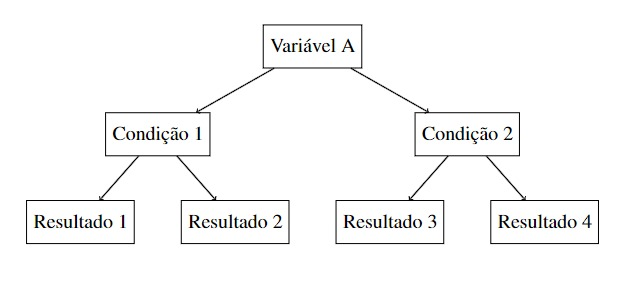
\includegraphics[width=0.7\textwidth]{arvore.png}
  \label{fig:funarvore}
\end{figure}
\begin{flushleft}
\vspace{-2em}
\centering
\source{Fonte: Elaborada pelo Autor, 2023}
\end{flushleft}



%\\ % Quebra de linha
%\vspace{1cm}

Neste exemplo, é apresentada uma estrutura básica de uma árvore de decisão. O nó raiz representa uma variável de interesse, enquanto os nós subsequentes representam diferentes condições ou critérios de decisão. Cada nó de decisão é conectado a dois ou mais nós de resultado, que representam as possíveis ações ou resultados decorrentes daquela condição específica. Nas  árvores de decisão  temos uma métrica chamada critério de decisão.
% final da arvore de decisão

\subsection{Critério de Decisão}

O critério em árvores de decisão é uma medida utilizada para determinar como os nós da árvore devem ser divididos durante a construção do modelo. O critério define a função de avaliação que determina qual divisão é considerada a melhor em termos de pureza das classes resultantes. 

Existem diferentes critérios utilizados em árvores de decisão, sendo os mais comuns o índice de Gini (Gini impurity) e a entropia. Esses critérios medem a impureza dos dados em um nó da árvore e procuram dividir o nó para reduzir a impureza e aumentar a homogeneidade das classes nós filhos.





\subsubsection{Índice de Gini}

O critério de Gini avalia a probabilidade de classificar incorretamente uma amostra aleatória com base na distribuição das classes em um nó. Ele mede a impureza dos dados, sendo que um valor de 0 indica que todas as amostras pertencem a uma única classe e um valor de 1 indica que as amostras estão igualmente distribuídas entre as classes. O índice de Gini pode ser obtido pela seguinte expressão:


\begin{equation}
    \text{Gini}(p) = 1 - \sum_{i=1}^{K} p_i^2,
\end{equation}

%\[
%\text{Gini}(p) = 1 - \sum_{i=1}^{K} p_i^2
%\]



 \noindent onde, $p$ representa a distribuição de probabilidade das classes em um nó,  %$i$ varia de $1$ a $K$, 
e $K$ é o número de classes. Para realizar o cálculo do índice de Gini, é necessário seguir alguns passos. Primeiramente, é preciso calcular o quadrado das probabilidades de cada classe, representadas por $p_i^2$. Em seguida, esses valores são somados. Por fim, o resultado dessa soma é subtraído de 1.

%Para calcular o índice de Gini, primeiro calculamos o quadrado das probabilidades de cada classe $p_i^2$, somamos esses valores e, em seguida, subtraímos o resultado de 1.  

%O índice de Gini varia de 0 a 1, onde um valor de 0 indica que todas como propriedade pertencem a uma única classe, ou seja, o nó é completamente puro. Um valor de 1 indica que as amostras estão igualmente distribuídas entre as classes, ou seja, o nó é impuro.

%Para realizar o cálculo do índice de Gini, é necessário seguir alguns passos. Primeiramente, é preciso calcular o quadrado das probabilidades de cada classe, representadas por $p_i^2$. Em seguida, esses valores são somados. Por fim, o resultado dessa soma é subtraído de 1.

O índice de Gini é uma medida que varia de 0 a 1. Quando o valor é igual a 0, significa que todas as propriedades pertencem a uma única classe, indicando que o nó é completamente puro. Por outro lado, quando o valor é igual a 1, isso indica que as amostras estão igualmente distribuídas entre as classes, tornando o nó impuro.


\subsubsection{Entropia}

A entropia, por sua vez, é uma medida de desordem ou incerteza nos dados. Ela é calculada com base na distribuição das classes em um nó e mede a impureza dos dados. Assim como o critério de Gini, a entropia é maximizada quando as classes estão igualmente distribuídas e minimizada quando todas as amostras pertencem a uma única classe. A entropia é uma medida utilizada em árvores de decisão para quantificar a impureza dos dados em um nó,  ela representa a quantidade de informação aleatória ou incerteza presente em um conjunto de dados. A fórmula do índice de entropia calcula a entropia de um conjunto de dados com base na distribuição das classes presentes.  De acordo com   \citeonline{arvore}, A medida de entropia busca, então, medir o grau de incerteza presente em cada esquema finito. A entropia pode ser obtida através da seguinte expressão: 


\begin{equation}
    \text{H(X)} = -\sum_{i=1}^{n} p(x_i) \log_{2} p(x_i),
\end{equation}

%\[
%\text{H(X)} = -\sum_{i=1}^{n} p(x_i) \log_{2} p(x_i)
%\]

%\begin{itemize}

%\item $H(X)$:  representa a entropia do conjunto de dados X;
%\item $n$:  é o número de classes distintas presentes no conjunto de dados; 
%\item $x_i$:  refere-se a uma classe específica dentro das n classes do conjunto de dados;
%\item $p(x_i)$:  é a probabilidade de ocorrência da classe $x_i$ no conjunto de dados X. Essa probabilidade é calculada dividindo o número de amostras que pertencem à classe $x_i$ pelo número total de amostras no conjunto de dados; 




\noindent em que a entropia é denotada por $H(X)$, sendo uma medida da incerteza ou desordem presente em um conjunto de dados chamado X. Quanto maior a entropia, maior a incerteza e a falta de informação sobre as classes presentes no conjunto de dados. O valor de $n$ representa o número de classes distintas encontradas em X, ou seja, é a quantidade de categorias diferentes que as amostras podem pertencer. Cada classe é denotada por $x_i$, onde $i$ é um índice que varia de 1 a n. A probabilidade de ocorrência de uma classe específica $x_i$ em X é representada por $p(x_i)$, essa probabilidade é calculada dividindo o número de amostras que pertencem à classe $x_i$ pelo número total de amostras presentes em X. Portanto, $p(x_i)$ fornece uma medida de quão frequente ou comum é a classe $x_i$ no conjunto de dados.



%\item $\log_{2} p(x_i)$:  representa o logaritmo na base 2 da probabilidade $p(x_i)$. O logaritmo é usado para calcular a contribuição de cada classe para a entropia total; 
%\item $\sum_{i=1}^{n}$:  indica a soma de todos os termos para cada classe $x_i$ no intervalo de $1$ a $n$. 
%\end{itemize}

A equação calcula a entropia somando as contribuições de cada classe ponderadas pela probabilidade de ocorrência da classe. Quanto mais homogêneo for o conjunto de dados (com todas as amostras pertencendo a uma única classe), menor será a entropia e, consequentemente, maior será a pureza do nó. Por outro lado, se as amostras estiverem igualmente distribuídas entre as classes, a entropia será máxima, indicando alta impureza ou incerteza. 

Ao construir uma árvore de decisão, o objetivo é reduzir a entropia dos nós ao máximo possível através da escolha de divisões que resultem em conjuntos de dados mais homogêneos em termos de classes. O critério de entropia é usado para determinar a divisão ótima em cada nó da árvore, buscando maximizar a informação ganha ao realizar a divisão.



\vspace{\onelineskip}

\section{Random Forest}

\vspace{\onelineskip}

De acordo  com \citeonline{avaliacao},   o \textit{Random Forest} é um método de aprendizado conjunto para classificação e regressão que opera construindo várias árvores de decisão no momento do
treinamento e produzindo a classe, que é o modo das saídas geradas por árvores individuais. O \textit{Random Forest} é um modelo de aprendizado de máquina que combina a ideia de árvores de decisão com o conceito de conjunto de modelos. O \textit{Random Forest} é composta por um conjunto de árvores de decisão individuais. Cada árvore é treinada independentemente em uma amostra aleatória dos dados de treinamento, e as previsões são feitas pela combinação das previsões de todas as árvores. Essa abordagem de conjunto ajuda a reduzir o viés e a variância do modelo, melhorando seu desempenho e capacidade de generalização.

Uma das características distintivas da \textit{Random Forest} é o uso de duas formas de aleatoriedade: a seleção aleatória dos dados de treinamento para cada árvore e a seleção aleatória das características (ou atributos) considerados em cada divisão da árvore. Essas fontes de aleatoriedade garantem que cada árvore seja treinada de forma independente e diversa, evitando o sobreajuste e aumentando a robustez do modelo.

O processo de construção de uma \textit{Random Forest} ocorre em várias etapas. Primeiro, é feita uma amostragem aleatória com substituição, conhecida como amostragem de \textit{bootstrap}. Assim como no \textit{bagging}, todas as amostras \textit{bootstrap} são identicamente distribuídas.
Isto implica que a esperança da média das B árvores é a mesma que a esperança de cada
uma delas, ou seja, o viés do modelo de árvores agregadas será equivalente ao observado
em cada árvore \cite{faelforest}. Após a seleção da amostra, uma árvore de decisão é treinada nessa amostra, mas em cada divisão da árvore, apenas um subconjunto aleatório de características é considerado. Esse processo de amostragem e treinamento é repetido para cada árvore na floresta.

Para fazer previsões por meio da \textit{Random Forest}, cada árvore individual produz uma previsão e a classe ou valor final é determinado por meio de uma combinação dos resultados das árvores. Para classificação, uma votação majoritária é usada para determinar a classe prevista, enquanto para regressão, uma média dos valores previstos é calculada. Essa abordagem de conjunto permite que o modelo aproveite a diversidade das árvores e forneça previsões mais precisas e estáveis.

A \textit{Random Forest} tem uma ampla gama de aplicações em diferentes áreas. É frequentemente usada para problemas de classificação, como detecção de fraudes em cartões de crédito, diagnóstico médico, análise de sentimentos e detecção de spam. Além disso, é aplicada em tarefas de regressão, como previsão de preços imobiliários, previsão de demanda e análise de séries temporais. Sua flexibilidade, robustez e capacidade de lidar com conjuntos de dados complexos tornam-na uma escolha popular em muitos cenários de aprendizado de máquina.

%Podemos afirmar que o \textit{Random Forest} é um modelo de aprendizado de máquina baseado em conjuntos que combina várias árvores de decisão. Sua aleatoriedade controlada e a combinação dos resultados das árvores proporcionam um modelo mais robusto e preciso. A \textit{Random Forest} tem diversas aplicações práticas e é especialmente útil em problemas de classificação e regressão. Compreender os princípios básicos e as características da Random.  Vale destacar que o modelo de Random Forest pode ser utilizado para resolver tanto problemas de regressão quanto problemas de classificação. A principal diferença entre os dois casos está na formulação geral do algoritmo, que pode sofrer algumas alterações, dependendo do tipo de problema que estamos enfrentando.


%Vale lembrar que este modelo pode ser usado tanto para problemas de regressão quanto para problemas de classificação  onde a formula geral acaba sofrendo algumas alterações dependendo do problema.




%\subsection{Random Forest  para Regressão}

%Ao contrário da Random Forest para classificação, onde a previsão final é determinada por meio de votação majoritária das árvores, a Random Forest para regressão utiliza uma média ou mediana das previsões de todas as árvores como valor final. Essa média ou mediana representa a estimativa do valor de regressão para uma determinada instância de entrada, a Random Forest para regressão é definida pela seguinte expressão:

%\vspace{\onelineskip}

%\begin{equation}
%    \hat{y} = \frac{1}{N} \sum_{i=1}^{N} h_i(x),
%\end{equation}

%\vspace{\onelineskip}
%\[
%\hat{y} = \frac{1}{N} \sum_{i=1}^{N} h_i(x)
%\]

%Nessa fórmula,
%\noindent em que $\hat{y}$ representa o valor previsto para a entrada $x$, $N$ é o número de árvores na floresta e $h_i(x)$ é a previsão da árvore $i$ para $x$. A média das previsões de todas as árvores é calculada, fornecendo a previsão final da Random Forest para o problema de regressão.


\subsection{Random Forest  Para Classificação}

A Random Forest para classificação utiliza um conjunto de árvores de decisão independentes que são treinadas em diferentes amostras aleatórias do conjunto de dados de treinamento. Cada árvore faz uma previsão de classe para uma instância de entrada com base em suas características. A fórmula do Random Forest na classificação é dada por:


\begin{equation}
    \hat{y} = \arg\max \left( \sum_{i=1}^{N} \mathbb{I}(h_i(x) = c) \right),
\end{equation}

%\[
%\hat{y} = \arg\max \left( \sum_{i=1}^{N} \mathbb{I}(h_i(x) = c) \right)
%\]

%\begin{itemize}
    %\item \(\hat{y}\) representa a classe prevista para a entrada \(x\);
   % \item \(\underset{}{\text{argmax}}\) significa que estamos buscando o valor de \(c\) que maximiza a expressão que segue;
  %  \item \(\sum_{i=1}^{N}\) é a soma sobre todas as \(N\) árvores da Random Forest;
   % \item \(h_i(x)\) é a previsão da árvore \(i\) para a entrada \(x\);
   % \item \(\mathbb{I}(h_i(x) = c)\) é uma função indicadora que retorna 1 se a previsão da árvore \(i\) para \(x\) for igual à classe \(c\), e 0 caso contrário.
%\end{itemize}

\noindent  em que $\hat{y}$ representa a classe prevista para a entrada \(x\),
$\underset{}{\text{argmax}}$ significa que estamos buscando o valor de \(c\) que maximiza a expressão que segue,
\(\sum_{i=1}^{N}\) é a soma sobre todas as \(N\) árvores da Random Forest,
\(h_i(x)\) é a previsão da árvore \(i\) para a entrada \(x\),
\(\mathbb{I}(h_i(x) = c)\) é uma função indicadora que retorna 1 se a previsão da árvore \(i\) para \(x\) for igual à classe \(c\), e 0 caso contrário. \\
 
A fórmula representa o processo de votação majoritária na Random Forest para determinar a classe prevista. Para cada classe possível \(c\), a soma conta quantas vezes a previsão da árvore \(i\) para a entrada \(x\) é igual a \(c\). A classe \(c\) que possui a maior soma é escolhida como a classe prevista para \(x\).  %Além dos modelos utilizados ,alguns métodos também foram aplicados como: seleção de atributos, undersampling, weighting balancing.



\vspace{\onelineskip}

\section{XGBoost}
\vspace{\onelineskip}
%\subsection{ O que é o Extreme Gradient Boosting (XGBOOST) }
%\vspace{\onelineskip}

O  \textit{Extreme Gradient Boosting} (XGBoost) é um algoritmo de aprendizado de máquina que se baseia no método de impulso (boosting) para criar modelos preditivos. O XGBoost  Segundo \citeonline{Iaexpert},   foi apresentado em 2016 por Tianqi Chen e Carlos Guestrin na Conferência SIGKDD e, desde então, tem sido o método de preferência dos profissionais da área.

%Ele foi desenvolvido por Tianqi Chen e é conhecido por sua eficácia e desempenho em competições de ciência de dados e aprendizado de máquina. 

 Esse método busca melhorar o desempenho do \textit{gradient boosting} otimizando a utilização do software (conhecimento técnico dos chefs) e hardware (ferramentas que eles usam para avaliar, como seus sentidos). Seria como criar um ambiente perfeito para que os avaliadores possam fazer o melhor trabalho possível: a nota mais factível no menor tempo. Digamos que os chefs recebem antecipadamente uma relação descritiva dos critérios a serem considerados, e um despalatizante para usarem entre as provas gustativas \cite{Iaexpert}.  

Existem várias razões pelas quais o XGBoost se tornou popular, Ele possui uma eficiência computacional significativa, sendo capaz de lidar com grandes conjuntos de dados e ter um bom desempenho. Além disso, o XGBoost utiliza técnicas avançadas de regularização para evitar o overfitting (sobreajuste) do modelo, o que o torna mais geral e robusto em relação a dados novos.


\begin{equation}
    \text{Obj}(\theta) = \sum_{i=1}^{n} l(y_i, \hat{y}_i) + \sum_{k=1}^{K} \Omega(f_k),
\end{equation}


%\[
%\text{Obj}(\theta) = \sum_{i=1}^{n} l(y_i, \hat{y}_i) + \sum_{k=1}^{K} \Omega(f_k),
%\]

%onde : 

%\begin{itemize}
%\item $\text{Obj}(\theta)$: é a função objetivo a ser otimizada;
%\item  $\theta$: são os parâmetros do modelo;
%\item  $n$: é o número de amostras de treinamento;
%\item $l(y_i, \hat{y}_i)$: é a função de perda que mede a diferença entre o valor verdadeiro $y_i$ e o valor predito  $\hat{y}_i$.
%\end{itemize}
  


%A função objetivo a ser otimizada é representada por $\text{Obj}(\theta)$. $\theta$ denota os parâmetros do modelo em questão. O número de amostras de treinamento é denotado por $n$. A função de perda, $l(y_i, \hat{y}_i)$, é usada para medir a diferença entre o valor verdadeiro $y_i$ e o valor predito $\hat{y}_i$.
\noindent em que a função objetivo a ser otimizada é representada por $\text{Obj}(\theta)$, $\theta$ são os parâmetros do modelo em questão,  $n$ é o número de amostras de treinamento. Utilizamos a função de perda $l(y_i, \hat{y}_i)$ para medir a diferença entre o valor verdadeiro $y_i$ e o valor predito $\hat{y}_i$, ou seja, basicamente a função de perda é o erro associado ao modelo durante o treinamento e é usada como uma medida de desempenho para ajustar o modelo para obter os melhores resultados possíveis. Por último, \(\Omega(f_k)\) é a função de penalidade ou regularização aplicada à árvore \(f_k\). Essa função tem como objetivo evitar overfitting e melhorar a generalização do modelo.




\vspace{\onelineskip}

\section{Suport Vector Machine}

\vspace{\onelineskip}


O  objetivo  do  algoritmo  da  máquina  de  vetores  de  suporte  (SVM –Support Vector Machine) é encontrar um hiperplano em um espaço N-dimensional (N -o número de recursos ou atributos) que classifica distintamente os pontos de dados \cite{datascienceacademy}. Segundo  \citeonline{suport}, é uma técnica de classificação que procura encontrar um hiperplano que particione os dados por seus rótulos de classe e ao mesmo tempo, evite o ajuste excessivo dos dados maximizando a margem da separação
hiperplano.  Na Figura \ref{fig:imagem1} podemos visualizar a definição do hiperplano:

%imagem   supurte vector machine  

%\vspace{1cm}

\begin{figure}[H]
  \centering
    \caption[Otimização do Hiperplano]{Otimização do Hiperplano}
  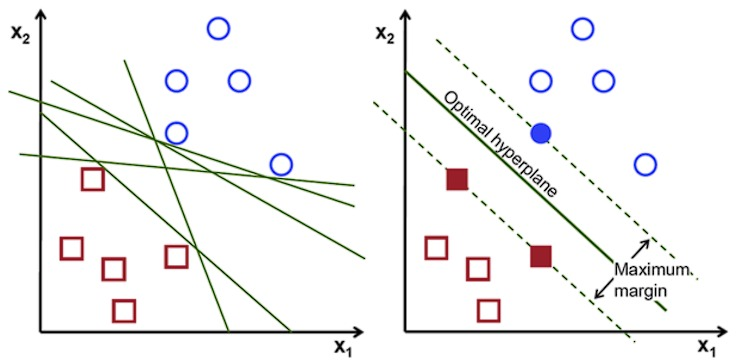
\includegraphics[width=0.7\textwidth]{whatsap_SVM.jpeg}
  \label{fig:imagem1}
\end{figure}
\begin{flushleft}
\vspace{-1.5em}
\centering
\source{Fonte: Data Science Academy(2022)}
\end{flushleft}
%\vspace{1cm}



%O objetivo é encontrar um hiperplano com a margem máxima, ou  seja,  a  distância  máxima  entre  os  pontos  de  dados  das  duas  classes. O modelo SVM pode ser aplicado tanto para dados  linearmente separáveis  (se tornando um problema de regressão) como também para dados não lineares (se tornando um problema de classificação). Para probelmas de classificação o modelo utilizará o truque de kernel, que envolve mapear os dados do espaço original de características para um espaço de alta dimensionalidade, onde seja possível alcançar uma melhor separação entre as classes.  Essa transformação é realizada através de uma função kernel, que calcula o produto interno entre dois pontos no espaço de alta dimensionalidade sem a necessidade de calcular explicitamente as coordenadas nesse espaço. Com o uso do truque de kernel, o SVM pode encontrar um hiperplano de separação ótimo mesmo em casos onde as classes não são linearmente separáveis no espaço original.




O objetivo é encontrar um hiperplano com a margem máxima, ou seja, a  distância  máxima  entre  os  pontos  de  dados  das  duas  classes. O modelo SVM pode ser aplicado tanto para dados linearmente separáveis (se tornando um problema de regressão) como também para dados não lineares (se tornando um problema de classificação). Para problemas de classificação, o modelo utilizará o truque de kernel, que envolve mapear os dados do espaço original de características para um espaço de alta dimensionalidade, onde seja possível alcançar uma melhor separação entre as classes.  Essa transformação é realizada por meio de uma função kernel, que calcula o produto interno entre dois pontos no espaço de alta dimensionalidade sem a necessidade de calcular explicitamente as coordenadas nesse espaço. Com o uso do truque de kernel, o SVM pode encontrar um hiperplano de separação ótimo mesmo em casos onde as classes não são linearmente separáveis no espaço original.




%Seja um conjunto de dados \(D\) rotulado como "positivo" e "negativo", em um espaço de características \(X\) de dimensão \(d\). O hiperplano \(H\) pode ser definido por uma função linear:


  % \begin{equation}
% \[ f(x) = \mathbf{w}^T \cdot \mathbf{x} + b \]
 %  \end{equation}


%onde:
%%- \(h(x)\) é a função de decisão que mapeia um dado de entrada \(x \in X\) para sua classe predita (positivo ou negativo).
%- \(\mathbf{w} \in \mathbb{R}^d\) é o vetor de pesos (ou coeficientes) do hiperplano.
%- \(\mathbf{x} \in \mathbb{R}^d\) é o vetor de características de entrada.
%- \(b \in \mathbb{R}\) é o termo de viés (\textit{bias}) que controla o deslocamento do hiperplano.

%O objetivo é encontrar os valores ideais para \(\mathbf{w}\) e \(b\) de modo que o hiperplano \(H\) maximize a margem entre os pontos positivos e negativos, ou seja, minimize a probabilidade de erro de classificação.  Podemos formular o problema de maximização da margem como uma tarefa de otimização convexa, onde a função objetivo é a largura da margem. 


% De acordo com 

    



%$$\subsection{Dados Não Lineares}




\subsection{Kernel Linear}





O SVM de kernel linear é um tipo de SVM em que se utiliza um kernel linear para mapear os dados de entrada em um espaço de maior dimensionalidade, onde é mais fácil separar as classes por meio de um hiperplano linear. O hiperplano linear é uma fronteira de decisão que separa os exemplos de diferentes classes.  Uma das principais vantagens do SVM de kernel linear é sua eficiência computacional, especialmente quando comparado a outros kernels mais complexos. A natureza linear do kernel permite que o SVM seja treinado e usado em grandes conjuntos de dados com menor tempo de processamento. Além disso, o SVM de kernel linear é menos suscetível a overfitting, o que ocorre quando o modelo se ajusta muito aos dados de treinamento e não generaliza bem para dados não vistos.

No entanto, o kernel linear é eficaz apenas quando os dados são linearmente separáveis. Caso contrário, o hiperplano linear não será capaz de separar completamente as classes, resultando em um desempenho inferior. Os dados não lineares nada mais são do que dados que não  se consegue dividir por meio de  uma reta, em outras palavras, não é possível traçar uma linha reta que represente de forma precisa a relação entre as variáveis em estudo, é possível perceber essa relação na Figura~\ref{fig:imagem} a seguir:
 %\vspace{1cm}

\begin{figure}[ht]
  \centering
\caption[Dados Não Lineares]{Dados Não Lineares}
  \includegraphics[width=0.5\textwidth]{dados_nao_lineares.jpeg}

  \label{fig:imagem}
\end{figure}
\begin{flushleft}
\vspace{-1.5em}
\centering
\source{Fonte: Data Science Academy(2022)}
\end{flushleft}

 %\vspace{1cm}


Ao contrário dos dados lineares, onde uma relação linear pode ser estabelecida usando uma equação matemática simples (por exemplo, $y = mx + b$), os dados não lineares requerem uma abordagem mais complexa para entender e modelar a relação entre as variáveis. Uma forma de contornar essa situação é  
usar a função de Kernel polinomial. 


\subsection{Kernel Polinomial}


O kernel polinomial é um tipo de kernel utilizado no algoritmo de Support Vector Machine (SVM) que permite mapear os dados de entrada em um espaço de maior dimensionalidade usando funções polinomiais. O kernel polinomial é usado quando os dados não são linearmente separáveis no espaço de entrada original. Ele transforma os dados de entrada em um espaço de maior dimensionalidade, onde pode ser possível encontrar um hiperplano linear que separe as classes. A função polinomial é aplicada aos pares de atributos dos dados, gerando novas características que representam as interações polinomiais entre os atributos.

A principal vantagem do kernel polinomial é sua capacidade de capturar relações não lineares entre os atributos. Ao elevar os atributos a potências mais altas, o kernel polinomial permite que o SVM modele separações mais complexas. A escolha adequada do grau do polinômio é crucial, pois um grau muito baixo pode não ser capaz de separar corretamente as classes, enquanto um grau muito alto pode levar a overfitting e dificuldades computacionais.

Uma desvantagem do kernel polinomial é que, à medida que o grau do polinômio aumenta, o número de características geradas também aumenta exponencialmente. Isso pode levar a problemas de alta dimensionalidade, especialmente quando o número de atributos originais já é grande. O aumento na dimensionalidade dos dados pode aumentar o tempo de treinamento e tornar o modelo mais suscetível ao overfitting.

O kernel polinomial tem várias aplicações práticas. É comumente usado em tarefas de classificação de imagem, como reconhecimento facial, detecção de objetos e segmentação de imagens. Também é aplicado em problemas de processamento de linguagem natural, como classificação de texto e análise de sentimentos. O kernel polinomial pode ser usado em qualquer problema onde as relações não lineares entre os atributos são importantes para a separação das classes. %embora seja amplamente utilizado em problemas de classificação de imagem, processamento de linguagem natural e outros domínios onde as relações não lineares são cruciais para a separação das classes.

%Logo, o kernel polinomial é um tipo de kernel usado no SVM para modelar relações não lineares entre os atributos dos dados. Ele mapeia os dados em um espaço de maior dimensionalidade usando funções polinomiais. Além disso, esse tipo de kernel é capaz de capturar separações mais complexas, mas pode levar a problemas de alta dimensionalidade e overfitting,


O kernel polinomial é definido como

%\begin{equation*}
% \[ K(x, y) = (\langle x, y \rangle + c)^d \]        
%\end{equation*}

\begin{equation}
    K(x, y) = (\langle x, y \rangle + c)^d,
\end{equation}
%    K(x, y) = (\langle x, y \rangle + c)^d;
%\end{equation}


\noindent em que $x$ e $y$ representam os vetores de entrada (dados), $\langle x, y \rangle$ é o produto interno entre os vetores, $c$ é um termo de deslocamento (bias) e $d$ é o grau do polinômio. A função do kernel polinomial consiste em elevar o produto interno dos vetores $x$ e $y$ a potência $d$, somar o termo de deslocamento $c$ e obter o resultado.



\vspace{\onelineskip}
\section{Seleção de Atributos}
%\vspace{\onelineskip}
\vspace{\onelineskip}
%\subsection{O que é Seleção de Atributos}

A seleção de atributos é um processo importante no campo do aprendizado de máquina. Trata-se de escolher os atributos mais relevantes de um conjunto de dados para melhorar o desempenho dos modelos de machine learning. Existem diferentes abordagens e métodos para realizar essa seleção. Segundo \citeonline{atributos},  o processo de seleção de características (FS)  permite reduzir a dimensionalidade dos dados, eliminando atributos redundantes e irrelevantes, reduzindo assim a complexidade dos modelos de previsão.

Uma forma de seleção de atributos é utilizando métodos embutidos, nos quais o algoritmo de aprendizado de máquina atribui importância aos atributos durante o treinamento. Por exemplo, o algoritmo Random Forest avalia a importância de cada atributo com base em sua contribuição para a redução da impureza nos nós das árvores de decisão. Além disso, existem técnicas de busca que exploram um espaço de soluções em busca do subconjunto de atributos que otimiza um critério específico. Essas técnicas podem ser exaustivas ou utilizar algoritmos heurísticos para encontrar a melhor combinação de atributos. A seleção de atributos é uma etapa importante no processo de modelagem de machine learning, pois ajuda a reduzir a dimensionalidade dos dados, evitar overfitting e melhorar a interpretabilidade do modelo. A escolha da abordagem e do método depende do contexto e dos requisitos específicos do problema.

%Outra abordagem é a utilização de métodos baseados em filtros, que avaliam os atributos independentemente do modelo de machine learning a ser utilizado. Esses métodos utilizam medidas estatísticas, como correlação ou ganho de informação, para classificar os atributos de acordo com sua relevância. Há também os métodos baseados em wrappers, que envolvem a avaliação do desempenho do modelo com diferentes subconjuntos de atributos. Eles selecionam o conjunto de atributos que resulta no melhor desempenho do modelo, mas podem exigir mais recursos computacionais.



\vspace{\onelineskip}
\section{  Valor de Shapley }
\vspace{\onelineskip}
%\vspace{\onelineskip}
%\subsection{Teoria do Valor de Shapley }
 Segundo \citeonline{bezerra_grande_silva_2009}, o conceito de valor neste caso não deve ser confundido com o conceito de valor apregoado pela economia,
A teoria do valor de Shapley foi desenvolvida por \citeonline{shapley1953value}, um matemático e economista norte-americano.  Os atributos Shapley foram inicialmente propostos por Shapley como uma medida de atribuição justa e equitativa de valores em jogos cooperativos, onde os jogadores contribuem de maneira conjunta para alcançar um resultado coletivo. A teoria ganhou importância em diversos campos, incluindo a economia, a ciência da computação e a análise de dados.  Ao calcular os atributos Shapley, é necessário considerar todas as combinações possíveis de variáveis e suas contribuições, a fim de alcançar uma distribuição justa do valor total.

 No contexto da análise de dados e aprendizado de máquina, os atributos Shapley podem ser aplicados para explicar as previsões de um modelo. Eles atribuem um valor a cada variável de entrada, indicando sua importância relativa na previsão do modelo. Essa abordagem proporciona uma compreensão mais profunda dos fatores que influenciam as previsões e auxilia na identificação das variáveis que exercem um impacto significativo.  Ao atribuir valores aos atributos Shapley, é possível identificar quais variáveis têm um impacto mais significativo nas previsões do modelo. Isso permite compreender quais características ou variáveis têm maior influência na tomada de decisões do modelo e como elas contribuem para o resultado final.



\vspace{\onelineskip}

\section{Undersampling}

\vspace{\onelineskip}

Segundo  \citeonline{udersampling},  problema de desequilíbrio de dados, ocorre na tarefa de classificação sempre que o número de observações pertencentes a uma das classes, a classe majoritária, excede o número de observações pertencentes a uma das outras classes, a classe minoritária. De acordo com \citeonline{livroingles1},  \textit{undersampling} consiste em reduzir os dados eliminando exemplos pertencentes à classe majoritária com o objetivo de equalizar o número de exemplos de cada classe
Undersampling é uma técnica utilizada no campo do aprendizado de máquina para lidar com conjuntos de dados desbalanceados, nos quais uma classe é significativamente mais representada do que as outras. O objetivo do \textit{undersampling} é reduzir a quantidade de exemplos da classe majoritária, de modo a equilibrar a distribuição das classes. Essa técnica pode ser aplicada de diferentes maneiras. Uma abordagem comum é a remoção aleatória de exemplos da classe majoritária até que a proporção entre as classes seja adequada. Dessa forma, a quantidade de exemplos da classe majoritária é reduzida para que fique mais próxima da quantidade de exemplos da classe minoritária.

Cabe ressaltar que o \textit{undersampling} pode ser realizado de forma simples ou estratificada. No \textit{undersampling} simples, os exemplos são removidos aleatoriamente sem considerar sua relação com os demais exemplos. Já no \textit{undersampling} estratificado, busca-se manter uma distribuição equilibrada nas características dos exemplos remanescentes, preservando assim as informações relevantes da classe majoritária. É importante ressaltar que o \textit{undersampling} pode resultar na perda de informações importantes contidas nos exemplos removidos da classe majoritária. Portanto, sua aplicação deve ser cuidadosa, considerando o impacto na representatividade e na capacidade do modelo de generalizar os dados.


\vspace{\onelineskip}
\section{Curva de Característica de Operação do Receptor (ROC)}
%\subsection{Curva ROC}
\vspace{\onelineskip}

Segundo \citeonline{Curva},  A análise ROC (\textit{Receiver Operating Characteristic}) teve origem na teoria de decisão estatística e foi desenvolvida entre 1950 e 1960 para avaliar a detecção de sinais em radar e na psicologia sensorial.
A curva de característica de operação do receptor (ROC) é uma ferramenta amplamente utilizada na área de aprendizado de máquina e estatística para avaliar o desempenho de modelos de classificação binária. Ela é construída plotando a taxa de verdadeiros positivos (Sensibilidade) no eixo y versus a taxa de falsos positivos (1 - Especificidade) no eixo $x$.  Um modelo ideal terá uma curva ROC que se aproxima do canto superior esquerdo do gráfico, indicando uma alta sensibilidade (alta taxa de verdadeiros positivos) e uma baixa taxa de falsos positivos. Por outro lado, um modelo aleatório terá uma curva ROC que se assemelha a uma linha diagonal, indicando que sua capacidade de discriminar entre as classes é equivalente à chance aleatória.

A curva ROC também fornece uma medida de desempenho chamada Área Sob a Curva (AUC), que mede a capacidade de discriminação do modelo. O valor da AUC varia de 0 a 1, onde 1 representa um modelo perfeito e 0,5 indica um modelo que é tão bom quanto o acaso.  A curva ROC e a AUC são particularmente úteis quando os dados estão desequilibrados, ou seja, quando uma das classes é muito mais comum do que a outra. Elas permitem avaliar a capacidade de um modelo de classificar corretamente as instâncias da classe minoritária, mesmo em condições de desequilíbrio


\vspace{\onelineskip}
\section{Métricas de Avaliação}
\vspace{\onelineskip}

Para realizar uma análise precisa do desempenho do modelo, é essencial examinar os indicadores de desempenho relevantes. Essas métricas proporcionam uma avaliação quantitativa do desempenho do modelo em relação às tarefas específicas para as quais ele foi desenvolvido. A seguir, serão apresentadas as principais métricas utilizadas para avaliação dos modelos nesta monografia.


\begin{itemize}
 

\item \textbf{Precision (Precisão):} é a proporção de exemplos classificados corretamente como positivos em relação a todos os exemplos classificados como positivos (verdadeiros positivos + falsos positivos). Para cada classe, é calculada a precisão.

\item \textbf{Recall (Revocação):} é a proporção de exemplos classificados corretamente como positivos em relação a todos os exemplos que realmente são positivos (verdadeiros positivos + falsos negativos). Para cada classe, é calculado o recall.

\item \textbf{F1-score:} é a média harmônica entre precision e recall. É útil quando você deseja ter uma medida única que leve em consideração tanto a precisão quanto o recall. O F1-score é uma métrica comum para avaliar modelos de classificação.

\item \textbf{Support (Suporte):} é o número de ocorrências de cada classe no conjunto de dados.

\item \textbf{Accuracy (Acurácia):} é a proporção de exemplos classificados corretamente em relação a todos os exemplos. É uma medida geral de desempenho do modelo.

\item \textbf{Macro avg (Média Macro):} é a média das métricas para todas as classes, atribuindo igual peso para cada classe. Essa média dá a mesma importância para todas as classes, independentemente do tamanho.

\item \textbf{Weighted avg (Média Ponderada):} é a média das métricas para todas as classes, ponderada pelo suporte de cada classe. Essa média leva em consideração a distribuição de classes e é útil quando as classes têm diferentes quantidades de exemplos.

\end{itemize}


%%------------------------------------------------------------------------
%                Seção para os resultados e discussão

%\titlespacing{\subsection}{0pt}{*0}{*0}

\titlespacing{\chapter}{0pt}{*0}{*0}
%\titlespacing{\section}{0pt}{*0}{*0}

\chapter{Aplicação e Resultados}
\section{Resultados}

Em uma primeira abordagem, realizou-se a limpeza dos dados, excluindo variáveis que não seriam relevantes para o nosso modelo, como o identificador do hospital, nome da unidade de saúde, estado da unidade de saúde, dentre as variáveis excluídas. Em seguida,  foi feita a análise exploratória dos dados para identificar padrões e verificar o balanceamento da variável resposta, também conhecida como variável alvo.

%Após o tratamento dos dados, restaram inicialmente 468.994 observações, o que demonstra que há um conjunto de dados robusto. Para reduzir o tempo de processamento no treinamento do modelo, foi realizada a divisão do conjunto de dados.  Assim, uma parte dos dados foi reservada para treinar o modelo, enquanto a outra parte, que o modelo ainda não teve acesso, poderá ser utilizada no futuro para outros procedimentos que serão discutidos posteriormente. Essa divisão resultou em 50\% dos dados para espera (dados a serem utilizados futuramente) e 50\% para treino e teste.  Abaixo podemos observar na Figura~\ref{fig:base} a frequência da variável resposta.



Após o tratamento dos dados, restaram inicialmente 468.994 observações e 66 variáveis, cuja descrição está em anexo nesta monografia, o que evidencia a existência de um conjunto de dados robusto. Para reduzir o tempo de processamento durante o treinamento do modelo, optou-se por dividir o conjunto de dados. Dessa forma, uma parte dos dados foi reservada para treinar o modelo, enquanto a outra parte, à qual o modelo ainda não teve acesso, poderá ser utilizada futuramente em outros procedimentos, que serão discutidos posteriormente. Essa divisão resultou em 50\% dos dados destinados à espera (dados a serem utilizados no futuro) e 50\% para o treino e teste.  Vale ressaltar que a divisão do conjunto de dados foi realizada de forma randomizada, 
mantendo a proporção do conjunto de dados inicial. Ou seja, utilizamos uma subamostra do conjunto de dados original para reduzir o custo computacional, além de permitir a utilização dos dados de espera no futuro, caso seja necessário. 

Na Figura~\ref{fig:base}, é possível observar a frequência das classes do banco de dados em porcentagem:




\begin{figure}[H]
  \centering
   \caption[Proporção das Classes do Banco de Dados em Porcentagem]{Proporção das Classes do Banco de Dados em Porcentagem}
   \vspace{-1.5em}
  \includegraphics[width=0.7\textwidth]{dados_ori.png}
  \label{fig:base}
\end{figure}
\begin{flushleft}
\vspace{-1.5em}
\centering
\source{Fonte: Elaborada pelo Autor, 2023}
\end{flushleft}

Como pode ser observado, o conjunto de dados está bastante desbalanceado, sendo necessário fazer o balanceamento dos dados. É importante que o banco de dados reduzido mantenha a proporção equivalente ao conjunto de dados original, para que se possa aplicar corretamente os procedimentos.  

\vspace{\onelineskip}
\subsection{Após a Divisão dos Dados}

\vspace{\onelineskip}

Na Figura~\ref{fig:reduzido}, é possível observar a frequência das classes do dataset reduzido em porcentagem:








\begin{figure}[H]
  \centering
    \caption[Proporção das Classes em Porcentagem do Banco de Dados Reduzidos]{Proporção das Classes em Porcentagem do Banco de Dados Reduzidos}
   \vspace{-1.5em}
  \includegraphics[width=0.7\textwidth]{dados_div.png} 
  \label{fig:reduzido}
  \end{figure}
  \begin{flushleft}
\vspace{-2.2em}
\centering
\source{Fonte: Elaborada pelo Autor, 2023}
\end{flushleft}




Após a divisão dos dados em dados de espera e dados para treino e teste, no intuito de aumentar as informações sobre a classe minoritária (classe 3), então  dividimos mais  50\%  dos dados de espera, filtramos os valores que são equivalentes a classe 3, uniremos o dataset(banco de dados) que ficou como base reduzida ao dataset  filtrando com base na classe 3, após esse procedimento ficamos com  a seguinte proporção dos dados:


\begin{table}[htbp]
    \centering
  \caption[Tabela de Proporções do Dataset Para Treino e Teste]{Tabela de Proporções do Dataset Para Treino e Teste}
  %\vspace{-1.0em}
    \begin{tabular}{cc}
        \toprule
        \textbf{Classe} & \textbf{Proporção (\%)} \\
        \midrule
        1 & 2,33\% \\
        2 & 5,61\% \\
        3 & 1,43\% \\
        4 & 44,92\% \\
        5 & 45,72\% \\
        \bottomrule
    \end{tabular}
    \label{tab:proporcoes}
    \end{table}
 \begin{flushleft}
\vspace{-2.2em}
\centering
\source{Fonte: Elaborada pelo Autor, 2023}
\end{flushleft}

Embora tenham sido inseridos novos dados referentes à classe 3, pode-se perceber que a proporção referente a essa classe não aumentou significativamente. No entanto, isso já era esperado devido ao desbalanceamento substancial no volume de dados. Agora, é possível prosseguir para o próximo passo, que consiste em executar o \textit{undersampling} nos dados.

\vspace{\onelineskip}
\subsection{Aplicando o Undersampling}
\vspace{\onelineskip}

Conforme discutido anteriormente, o \textit{undersampling} é uma técnica utilizada no campo de aprendizado de máquina para tratar conjuntos de dados desbalanceados, nos quais uma ou mais classes estão significativamente sub-representadas em relação às outras. Nesse contexto, o \textit{undersampling} envolve a redução do número de amostras da classe majoritária (ou classes majoritárias) para equilibrar a distribuição das classes. Após aplicar a subamostragem, foram obtidas 15.390 observações, sendo 3.078 observações para cada classe. O próximo passo consiste em dividir os dados em conjuntos de treinamento e teste, a fim de prosseguir para a etapa de criação do modelo. %A partir desse ponto, foram utilizados exclusivamente pacotes e bibliotecas da linguagem Python, como sklearn, pandas, matplotlib, imblearn.under_sampling e xgboost.



%Após aplicar a subamostragem, foram obtidas 15.390 observações, sendo 3.078 observações para cada classe. O próximo passo consiste em dividir os dados em conjuntos de treinamento e teste, a fim de prosseguir para a etapa de criação do modelo.



\vspace{\onelineskip}
\subsection{Modelo 1: Árvore de Decisão}
\vspace{\onelineskip}

% O primeiro modelo será de árvore de decisão, é um modelo  bastante utilizado em problemas de classificação. Na Tabela~\ref{tab:my_label}, é possível observar as métricas do modelo de árvore de decisão.

O primeiro modelo utilizado será a árvore de decisão, um método amplamente empregado em problemas de classificação. O algoritmo  de árvore de decisão utilizado foi o  \textit{Classification and Regression Trees}(CART), Na Tabela~\ref{tab:my_label}, encontram-se as métricas referentes ao desempenho desse modelo:

\begin{table}[htbp]
    \centering
 \caption[Métricas do Modelo de Árvore de Decisão]{Métricas do Modelo de Árvore de Decisão}
    \begin{tabular}{cccccc}
        \toprule
        \textbf{Classe} & \textbf{Precisão} & \textbf{Revocação} & \textbf{F1-Score} & \textbf{Suporte} \\
        \midrule
        1 & 0,91 & 0,92 & 0,92 & 616 \\
        2 & 0,96 & 0,96 & 0,96 & 615 \\
        3 & 0,55 & 0,57 & 0,56 & 616 \\
        4 & 0,60 & 0,58 & 0,59 & 616 \\
        5 & 0,87 & 0,84 & 0,85 & 615 \\
        \midrule
        \textbf{Acurácia} & & & 0,78 & 3078 \\
        \textbf{Média (Macro)} & 0,78 & 0,78 & 0,78 & 3078 \\
        \textbf{Média Ponderada} & 0,78 & 0,78 & 0,78 & 3078 \\
        \bottomrule
    \end{tabular}

    \label{tab:my_label}
\end{table}
 \begin{flushleft}
\vspace{-2.2em}
\centering
\source{Fonte: Elaborada pelo Autor, 2023}
\end{flushleft}







Essa é uma matriz de resultados de classificação, conhecida como relatório de classificação ou classification report. Ele fornece várias métricas para avaliar o desempenho de um modelo de classificação.  Pode-se notar que o modelo apresenta um desempenho razoável, com uma acurácia de 78\%. As classes 1, 2 e 5 apresentam bons resultados, com precision, recall e F1-score acima de 85\%. Entretanto, As classes 3 e 4 têm resultados um pouco inferiores, com F1-score em torno de 56\% e 59\%, respectivamente.  Vamos criar outros modelos e verificar se os resultados melhoram.

%\begin{itemize}
 

%\item \textbf{Precision (Precisão):} é a proporção de exemplos classificados corretamente como positivos em relação a todos os exemplos classificados como positivos (verdadeiros positivos + falsos positivos). Para cada classe, é calculada a precisão.

%\item \textbf{Recall (Revocação):} é a proporção de exemplos classificados corretamente como positivos em relação a todos os exemplos que realmente são positivos (verdadeiros positivos + falsos negativos). Para cada classe, é calculado o recall.

%\item \textbf{F1-score:} é a média harmônica entre precision e recall. É útil quando você deseja ter uma medida única que leve em consideração tanto a precisão quanto o recall. O F1-score é uma métrica comum para avaliar modelos de classificação.

%\item \textbf{Support (Suporte):} é o número de ocorrências de cada classe no conjunto de dados.

%\item \textbf{Accuracy (Acurácia):} é a proporção de exemplos classificados corretamente em relação a todos os exemplos. É uma medida geral de desempenho do modelo.

%\item \textbf{Macro avg (Média Macro):} é a média das métricas para todas as classes, atribuindo igual peso para cada classe. Essa média dá a mesma importância para todas as classes, independentemente do tamanho.

%\item \textbf{Weighted avg (Média Ponderada):} é a média das métricas para todas as classes, ponderada pelo suporte de cada classe. Essa média leva em consideração a distribuição de classes e é útil quando as classes têm diferentes quantidades de exemplos.

%\end{itemize}





\vspace{\onelineskip}
\subsection{Modelo 2: Extreme Gradient Boosting (XGBoost)}
\vspace{\onelineskip}

 O segundo modelo será o XGboost,  também muito usando em problemas de classificação multiclasse.  Na Tabela~\ref{tab:xgboost}, é possível observar as métricas do modelo XGBoost:  


 


\begin{table}[H]
    \centering
    \caption[Métricas do Modelo XGBoost]{Métricas do Modelo XGBoost}
    \begin{tabular}{cccccc}
        \toprule
        \textbf{Classe} & \textbf{Precisão} & \textbf{Revocação} & \textbf{F1-Score} & \textbf{Suporte} \\
        \midrule
        1 & 0,99 & 0,93 & 0,95 & 616 \\
        2 & 0,96 & 0,99 & 0,98 & 615 \\
        3 & 0,67 & 0,57 & 0,62 & 616 \\
        4 & 0,64 & 0,75 & 0,69 & 616 \\
        5 & 0,91 & 0,92 & 0,92 & 615 \\
        \midrule
        \textbf{Acurácia} & & & 0,83 & 3078 \\
        \textbf{Média (Macro)} & 0,84 & 0,83 & 0,83 & 3078 \\
        \textbf{Média Ponderada} & 0,84 & 0,83 & 0,83 & 3078 \\
        \bottomrule
    \end{tabular}
    \label{tab:xgboost}
\end{table}
 \begin{flushleft}
\vspace{-1.5em}
\centering
\source{Fonte: Elaborada pelo Autor, 2023}
\end{flushleft}

Conforme observado, com o modelo XGBoost, houve melhorias nas métricas das classes 3 e 4. Além disso, o modelo apresenta métricas excelentes para as classes 1, 2 e 5. Isso indica que o modelo está desempenhando bem na classificação dessas classes específicas.    


\vspace{\onelineskip}
\subsection{Modelo 3: Suport Vector Machine}
\vspace{\onelineskip}


O terceiro modelo será o SVM com kenel polinomial também muito usando em problemas de classificação multiclasse. Na tabela~\ref{tab:SVM}, é possível observar as métricas do modelo SVM: 


\begin{table}[H]
    \centering
    \caption[Métricas do Modelo SVM Kenel Polinomial]{Métricas do Modelo SVM Kenel Polinomial}
    \begin{tabular}{cccccc}
        \toprule
        \textbf{Classe} & \textbf{Precisão} & \textbf{Revocação} & \textbf{F1-Score} & \textbf{Suporte} \\
        \midrule
        1 & 0,98 & 0,90 & 0,94 & 616 \\
        2 & 0,96 & 0,99 & 0,97 & 615 \\
        3 & 0,54 & 0,54 & 0,54 & 616 \\
        4 & 0,55 & 0,67 & 0,60 & 616 \\
        5 & 0,94 & 0,76 & 0,84 & 615 \\
        \midrule
        \textbf{Acurácia} & & & 0,77 & 3078 \\
        \textbf{Média (Macro)} & 0,79 & 0,77 & 0,78 & 3078 \\
        \textbf{Média Ponderada} & 0,79 & 0,77 & 0,78 & 3078 \\
        \bottomrule
    \end{tabular}

    \label{tab:SVM}
\end{table}
 \begin{flushleft}
\vspace{-1.0em}
\centering
\source{Fonte: Elaborada pelo Autor, 2023}
\end{flushleft}


Pode-se observar que o modelo SVM teve um desempenho inferior em relação aos modelos anteriores, especialmente nas classes 3 e 4.

\vspace{\onelineskip}
\subsection{Modelo 4: Random Forest}
\vspace{\onelineskip}

 O próximo modelo utilizado foi o Random Forest, Na Tabela~\ref{tab:forest}, é possível observar as métricas do modelo  Ramdom Forest: 


 \begin{table}[H]
    \centering
    \caption[Métricas do Modelo Random Forest ]{Métricas do Modelo Random Forest}
    \begin{tabular}{cccccc}
        \toprule
        \textbf{Classe} & \textbf{Precisão} & \textbf{Revocação} & \textbf{F1-Score} & \textbf{Suporte} \\
        \midrule
        1 & 1,00 & 0,90 & 0,95 & 616 \\
        2 & 0,91 & 0,99 & 0,95 & 615 \\
        3 & 0,66 & 0,45 & 0,54 & 616 \\
        4 & 0,58 & 0,82 & 0,68 & 616 \\
        5 & 0,93 & 0,86 & 0,89 & 615 \\
        \midrule
        \textbf{Acurácia} & & & 0,80 & 3078 \\
        \textbf{Média (Macro)} & 0,82 & 0,80 & 0,80 & 3078 \\
        \textbf{Média Ponderada} & 0,82 & 0,80 & 0,80 & 3078 \\
        \bottomrule
    \end{tabular}
    \label{tab:forest}
\end{table}
 \begin{flushleft}
\vspace{-1.0em}
\centering
\source{Fonte: Elaborada pelo Autor, 2023}
\end{flushleft}

 Pode-se notar que o modelo apresenta uma melhora em relação ao modelo Svm, entretanto, as métricas ainda estão abaixo do modelo XGBoost.


\vspace{\onelineskip}
\subsection{Modelo 5: XGBoost com Seleção de Atributos}
\vspace{\onelineskip}

 
  Na Tabela~\ref{tab:slection}  pode-se observar as métricas do XGBoost  com seleção de atributos:

\begin{table}[htbp]
    \centering
    \caption[Métricas do Modelo XGBoost com Seleção de Atibutos]{Métricas do Modelo XGBoost com Seleção de Atibutos}
    \begin{tabular}{cccccc}
        \toprule
        \textbf{Classe} & \textbf{Precisão} & \textbf{Revocação} & \textbf{F1-Score} & \textbf{Suporte} \\
        \midrule
        1 & 1,00 & 0,90 & 0,95 & 616 \\
        2 & 0,96 & 0,98 & 0,97 & 615 \\
        3 & 0,52 & 0,49 & 0,50 & 616 \\
        4 & 0,56 & 0,66 & 0,61 & 616 \\
        5 & 0,92 & 0,90 & 0,91 & 615 \\
        \midrule
        \textbf{Acurácia} & & & 0,78 & 3078 \\
        \textbf{Média (Macro)} & 0,79 & 0,79 & 0,79 & 3078 \\
        \textbf{Média Ponderada} & 0,79 & 0,78 & 0,79 & 3078 \\
        \bottomrule
    \end{tabular}

    \label{tab:slection}
\end{table}
 \begin{flushleft}
\vspace{-1.0em}
\centering
\source{Fonte: Elaborada pelo Autor, 2023}
\end{flushleft}


Pode-se notar que  o desempenho do modelo utilizando a  seleção de atributos teve  uma diminuição em sua performance geral, isso indica que  possivelmente, mesmos as covariáveis  não ter apresentando importância, elas provavelmente contribui de certa forma para a predição do modelo.





\subsection{Curva Roc}


Será feita a observação da curva ROC do melhor modelo, XGBoost(modelo: 2), o qual exibirá a curva ROC para cada classe. O XGBoost é amplamente reconhecido como um algoritmo eficiente e poderoso para problemas de classificação em aprendizado de máquina. A curva ROC é uma ferramenta valiosa para avaliar o desempenho de um modelo de classificação. Na Figura~\ref{fig:Roc} é possível observar os resultados obtidos:
 % pois mostra a taxa de verdadeiros positivos em relação à taxa de falsos positivos em diferentes limiares de classificação. 



\begin{figure}[H]
  \centering
   \caption[Curva Característica de Operação do Receptor(ROC)]{Curva Característica de Operação do Receptor(ROC)} 
  \includegraphics[width=0.7\textwidth]{curvaroc.png}
  \label{fig:Roc}
  \end{figure}
 \begin{flushleft}
\vspace{-1.0em}
\centering
\source{Fonte: Elaborada pelo Autor, 2023}
\end{flushleft}

  Embora os resultados obtidos pareçam satisfatórios, ela não é a métrica mais indicada para esse tipo de cenário. A curva ROC é amplamente utilizada em problemas de classificação binária, nos quais existem apenas duas classes a serem previstas. Ela representa a relação entre a taxa de verdadeiros positivos e a taxa de falsos positivos em diferentes limiares de classificação.  No entanto, ao lidar com problemas de multiclassificação, em que existem mais de duas classes, a curva ROC se torna menos informativa. A principal razão para isso é que a curva ROC é calculada para uma classe versus todas as outras, o que significa que é necessário realizar várias comparações para cada classe individualmente. Esse processo pode levar a uma análise complexa e menos clara do desempenho do modelo. Em vez disso, é preferível utilizar outras métricas mais apropriadas para problemas de multiclassificação como  foi apresentado na Tabela~\ref{tab:xgboost}. Além disso, outra forma de avaliar o modelo  é através    da matriz  de confusão.



\vspace{\onelineskip}
\subsection{Matriz de Confusão do Melhor Modelo}
\vspace{\onelineskip}

Na sequência, será feita a matriz de confusão para o modelo que obteve as melhores métricas, o modelo Extreme Gradient Boosting (XGBoost). A Tabela~\ref{tab:melhorxgbost} a seguir, apresenta as classificações feitas pelo modelo:






\begin{table}[H]
    \centering
    \caption[Matriz de Confusão do melhor modelo: XGBoost]{Matriz de Confusão do melhor modelo:
     XGBoost}
    \begin{tabular}{@{}cccccc@{}}
        \toprule
        & \textbf{Classe 1} & \textbf{Classe 2} & \textbf{Classe 3} & \textbf{Classe 4} & \textbf{Classe 5} \\
        \midrule
        \textbf{Classe 1} & 570 & 1 & 12 & 18 & 15 \\
        \textbf{Classe 2} & 0 & 609 & 1 & 0 & 5 \\
        \textbf{Classe 3} & 3 & 15 & 354 & 219 & 25 \\
        \textbf{Classe 4} & 3 & 0 & 140 & 464 & 9 \\
        \textbf{Classe 5} & 2 & 8 & 19 & 19 & 567 \\
        \bottomrule
    \end{tabular}
       \label{tab:melhorxgbost}
\end{table}
 \begin{flushleft}
\vspace{-1.0em}
\centering
\source{Fonte: Elaborada pelo Autor, 2023}
\end{flushleft}
 % Pode-se notar que de fato, as classes  1, 2 e 5 tiveram  boas classificações enquanto as classes 3 e 4  tiveram classificações moderadas, porém é notório  que as classificações erradas presentes nessas classes  se concentraram nelas, ou seja, por exemplo,  onde  a classe 4 foi classificada  incorretamente  o modelo a  classificou como sendo da classe 3 em pelo menos na maioria dos casos  e o mesmo aconteceu com a classe 3, que teve a maior parte das classificações erradas, sendo  considerada pelo modelo como a classe 4. 
 
 
 Pode-se observar que as classes 1, 2 e 5 obtiveram boas classificações, enquanto as classes 3 e 4 apresentaram classificações moderadas. É notável, no entanto, que os erros de classificação se concentraram nessas duas últimas classes. Por exemplo, quando o modelo classificou incorretamente um item como pertencente à classe 4, na maioria dos casos, ele o rotulou como pertencente à classe 3, e o mesmo ocorreu para a classe 3, onde a maioria das classificações erradas foi rotulada como classe 4 pelo modelo. Esses resultados sugerem uma proximidade nos atributos dessas duas classes encontrados durante a etapa de treinamento pelo modelo.



\subsection{Importância dos Atributos Shapley}


Por último, será gerado o gráfico de importância dos atributos para o modelo, utilizando o método dos atributos Shapley, que permitirá visualizar e analisar a contribuição individual de cada atributo na tomada de decisões do modelo. Isso fornecerá uma compreensão mais clara e detalhada de como cada variável influencia as previsões realizadas pelo modelo.  Na Figura~\ref{fig:Shaplay}  podemos ver a importância das covariáveis para o modelo XGboost:

 \begin{figure}[H]
  \centering

    \caption[Importância dos Atributos Shapley]{Importância dos Atributos Shapley} 
      \vspace{-0.75em}
  \includegraphics[width=0.7\textwidth]{importancia.png}

  \label{fig:Shaplay}
  \end{figure}
 \begin{flushleft}
\vspace{-1.9em}
\centering
\source{Fonte: Elaborada pelo Autor, 2023}
\end{flushleft}


 Pode-se observar na Figura~\ref{fig:Shaplay} acima, as 9 covariáveis que exercem o maior impacto nas predições do modelo. Entre elas, destacam-se POS\_PCROUT(Resultado da RTPCR foi positivo para outro vírus respiratório), PCR\_VSR (Resultado diagnóstico do RTPCR para (VSR))  , POS\_AN\_OUT(Resultado do Teste Antigênico, que foi positivo para outro vírus respiratório)  e  POS\_PCRFLU(Resultado da RTPCR foi positivo para Influenza), que apresentaram maior relevância para o modelo. É importante ressaltar que, apesar dessas 9 covariáveis serem as mais importantes, a interação entre os outros 56 atributos também desempenha um papel relevante para o  modelo.       
 %
 %as  10 covariáveis  que mais impactam  nas predições do modelo. POS\_PCROUT, PCR\_VSR,  POS\_PCRFLU,  POS\_PCRFLU   tiveram maior importancia para o modelo.   Embora  para o modelo essas 10 covariáveis tenham mais importância, de certa forma a  interação entre os outros 56 atributos  apresentam uma certa relevância para o modelo.



\chapter{Conclusão}

%Ao analisar os resultados obtidos, nota-se que o XGBoost apresentou melhores métricas de classificação para as 5 classes do que os demais modelos, obtendo uma perfomance geral de 83\%. No entanto, as classes 3 e 4 apresentaram uma performance apenas razoável, ficando apenas acima do aleatório. Esse fato pode ocorrer por vários motivos. Apesar de termos feito o balanceamento dos dados através do undersampling, equilibrando todas as classes, é provável que as classes 1, 2 e 5 possuam definições de seus atributos mais concretas. Já a classe 3 refere-se a  SRAG por outro agente etiológico, o que significa que pode haver mais de 3 agentes, o que pode influenciar na distribuição dos atributos pertencentes a essa classe, dificultando sua classificação. Algo semelhante ocorre com a classe 4, onde ela se refere a um tipo de SRAG que não foi capaz de ser especificado com base nos seus atributos.

%Conforme discutido anteriormente, é perceptível que, de forma geral, o modelo XGBoost apresentou resultados superiores em relação aos demais modelos. Isso confirma a eficácia do XGBoost na tarefa de classificação em comparação às outras abordagens consideradas.  Portanto, é o modelo mais indicado para prosseguir com a implementação. No entanto, antes disso, seria interessante tentar outras técnicas de processamento de dados, bem como de balanceamento e ajustes de modelo, para verificar se as métricas das classes 3 e 4 sofreram uma melhora. Uma performance melhor do modelo é o mais adequado, uma vez que estamos trabalhando na área da saúde.


Neste trabalho  foram  demonstradas algumas das principais técnicas de machine learning para classificação multiclasse, visando aprimorar a capacidade de previsão de síndromes respiratórias agudas graves (SRAG). Ao longo da pesquisa, foram utilizados diferentes modelos de classificação, sendo o XGBoost o que apresentou melhores resultados em relação às métricas de classificação para as cinco classes analisadas. Essa abordagem permitiu uma performance geral de 83\%, destacando-se especialmente na classificação de SRAG por influenza, SRAG por Covid, além das SRAGs por outros vírus respiratórios.  No entanto, as classes 3 e 4 demonstraram apenas uma performance razoável, ficando ligeiramente acima do nível aleatório. Essa ocorrência pode ser atribuída a diversos fatores. Embora tenhamos realizado o balanceamento dos dados através do undersampling, equilibrando todas as classes, é possível que as classes 1, 2 e 5 tenham definições mais concretas de seus atributos. Em contraste, a classe 3 abrange a SRAG por outros agentes etiológicos, o que pode significar a existência de múltiplos agentes, impactando a distribuição dos atributos e dificultando sua classificação. De maneira similar, a classe 4 refere-se a um tipo de SRAG que não pôde ser especificado com base em seus atributos. Consequentemente, embora o modelo XGBoost tenha apresentado desempenho geral superior em relação aos demais modelos, é necessário considerar o aprimoramento das métricas nas classes 3 e 4. Para prosseguir com a implementação, é recomendável explorar outras técnicas de processamento de dados, bem como estratégias adicionais de balanceamento e ajustes no modelo. Melhorar o desempenho do modelo é crucial, especialmente considerando o contexto da área de saúde


%Ao analisar os resultados obtidos, observa-se que o modelo XGBoost apresentou métricas de classificação superiores para as 5 classes em comparação com os demais modelos, alcançando uma performance geral de 83\%.


 Após analisar a matriz de confusão do melhor modelo, notou-se que a maioria das predições incorretas das classes 3 e 4 estava concentrada em sua proximidade, indicando uma forte semelhança entre os atributos (características) dessas duas classes. Isso pode ter contribuído para as dificuldades em distingui-las corretamente e resultou em um número maior de classificações equivocadas entre elas.  Com tudo, pode-se notar que, mesmo com as ressalvas, o modelo é capaz de prever com excelente performance a classificação de SRAG por influenza, SRAG por Covid, além das SRAGs por outros vírus respiratórios. Vale ressaltar que, quando estamos trabalhando em áreas como a saúde, é importante ter o menor erro possível, pois o erro pode custar vidas.

%%-----------------------------------------------------------------------
%                     ELEMENTOS PÓS-TEXTUAIS
\postextual

%%-----------------------------------------------------------------------
%                   Referências bibliográficas
\bibliography{bibliografias}



%\chapter{Anexo}

%\subsection{Anexo 1}
%\nopagebreak
%\subsection{Descrição das Variáveis Utilizadas}

%\subsection{Anexo A : Descrição das Variáveis Utilizadas}

%\vspace{-\baselineskip} % Remove espaço vertical extra antes da seção
%\begin{minipage}{\textwidth}
%\includepdf[pages=-, fitpaper]{anexos/descricao_variaveis.pdf}
%\end{minipage}
%\vspace{-\baselineskip} % Remove espaço vertical extra depois do minipage



%\begin{minipage}{\textwidth}
%\includepdf[pages=-, scale=0.9]{anexos/descricao_variaveis.pdf}
%\end{minipage}

%\includepdf[pages=-]{anexos/descricao_variaveis.pdf}

% adiciona o anexo  na mesma seção 
%\includepdf[pages=1,pagecommand=\section{Anexo A: Descrição das Variáveis Utilizadas}[ANEXO A: DESCRIÇÃO DAS VARIÁVEIS UTILIZADAS], offset=0 -3cm]{anexos/descricao_variaveis.pdf}
%\includepdf[pages=2-,pagecommand={}]{anexos/descricao_variaveis.pdf}


\includepdf[pages=1,pagecommand={\chapter{Anexo A: Descrição das Variáveis Utilizadas}}, offset=0 -3cm]{anexos/tabela.pdf}
\includepdf[pages=2-,pagecommand={}]{anexos/tabela.pdf}

%------------------------------------------------------------------------


%\subsection{Anexo 2 : Dicionário  dos Dados Completo}
%\nopagebreak

%\includepdf[pages=-]{anexos/Dicionario_compelto2.pdf}
% Adicione as duas páginas em branco
\newpage
\newpage
\end{document}
